% !TeX program = lualatex

\documentclass[12pt]{article}
\usepackage{placeins}
\usepackage{geometry}
\usepackage{subcaption}
\usepackage{wrapfig}

\newcommand{\mysub}[2][]% #1=caption (optional), #2=graphics
{\bgroup
  \sbox0{#2}\usebox0
  \dimen0=\dimexpr \textwidth-\wd0\relax
  \ifx\\\@centercr \divide\dimen0 by 2\fi
  \sbox1{\begin{minipage}[t]{\dimen0}
    \subcaption{#1}%
  \end{minipage}}%
  \rlap{\raisebox{\dimexpr \ht0-\ht1}[0pt][0pt]{\usebox1}}\allowbreak
\egroup}

\geometry{
	paper=a4paper, % Paper size
	top=2.5cm, % Top margin
	bottom=2.5cm, % Bottom margin
	left=2.5cm, % Left margin
	right=2.5cm, % Right margin
	headheight=0.75cm, % Header height
	footskip=1.5cm, % Space from the bottom margin to the baseline of the footer
	headsep=0.75cm, % Space from the top margin to the baseline of the header
	%showframe, % Uncomment to show how the type block is set on the page
}
\usepackage[english]{babel}
\usepackage[]{ragged2e}

\addto\captionsenglish{% Replace "english" with the language you use
  \renewcommand{\contentsname}%
    {Table of Contents}}

\usepackage{blindtext}
% \usepackage{background}
%-------------------------------- Character encoding ----------------------------
\usepackage[]{fontspec}
\usepackage[T1]{fontenc}
\setmainfont{Times New Roman}
%----------------------------- Mathematics packages from AMS ---------------

\usepackage{amsmath, amsfonts, amsthm, amssymb}
\usepackage{braket, nicefrac}

% ----------- International System of Units
\usepackage{siunitx}
\usepackage{tikz}

%------------------------------ Lists / numbers -------------------------
\usepackage{enumitem, multicol}

%------------------------------- Figure insertions --------------
\usepackage{graphicx, float}  % Use option [H] to force the placement of a figure
\usepackage{keystroke}
\usepackage{pgfplots}\usepgfplotslibrary{units}\pgfplotsset{compat=1.16}
\usepackage{fancyhdr}
\usepackage{eso-pic}

\usepackage{caption}
\usepackage{subcaption}
%------------------------------- Line Spacing --------------
\usepackage{setspace}

%------------------------------- Depth of the ToC --------------
\setcounter{tocdepth}{2}

%%%%%%%%%%%%%%%%%%%%%%%%%% Hyperlink References %%%%%%%%%%%%%%%%%%%%%%%%%%%
\usepackage[hidelinks]{hyperref}

%--------------------% Storage Path for images %-----------------%
\graphicspath{{figures/}{Graphics/}{./}}

\setcounter{tocdepth}{2}
\setcounter{secnumdepth}{4}


\pagestyle{fancy}
\fancyhf{}
\chead{FIGHTER UAV COMPETITION 2022}
\cfoot{METU Comet Astrotech}
\rfoot{\thepage}

\pagenumbering{gobble} % Title page
\begin{document}
\setstretch{1.15}


% \begin{figure}[ht]
% 	\centering
% 	\includegraphics[scale = 0.6]{}
% 	\caption{\label{fig:label} Caption.}
% \end{figure}


% \begin{table}[ht]
% 	\centering
% 	\csvautotabular{} değişebilir 
% 	\caption{\label{tbl:label} Caption.}
% \end{table}



\begin{titlepage}
    \centering
    
    \AddToShipoutPictureBG*{
    % \vspace{100pt}{
        \begin{tikzpicture}[opacity=0.3]
      \node {
\includegraphics[width=\pagewidth]{Comet_logo.png}}; \\
    %   \node {
\includegraphics[width=\pagewidth]{teknofest_logo.png}}; \\
            
        \end{tikzpicture}
        }

	\title{ %TODO texts can be made bigger
		TEKNOFEST \\
		AVIATION, SPACE AND TECHNOLOGY FESTIVAL \\
		FIGTHER UAV COMPETITION \\
		CRITICAL DESIGN REPORT \\}
	\author{
		TEAM NAME: \\ METU COMET ASTROTECH \\
		AUTHORS :\\ Ahmet NACAR\\ Alperen TEKİN\\ Fatma Ceyda GÖKÇE\\ Fethullah CEYLAN\\ Furkan ÇİTİL\\ Gamze ÇELİK\\ Göktuğ Mete KESİCİ \\ Metehan ATCI \\ Shaikh Muhammad ADIL \\ Zafer Doğan BUDAK} %TODO Authors to be added
	\date{}
	\maketitle
\end{titlepage}	
\clearpage
    \AddToShipoutPictureBG{
    % \vspace{100pt}{
        \begin{tikzpicture}[opacity=0.3]
    %   \node {
\includegraphics[width=\pagewidth]{Comet_logo.png}}; \\
      \node {
\includegraphics[width=\pagewidth]{teknofest_logo.png}}; 
            
        \end{tikzpicture}
        }

% \noBgThispage
\pagenumbering{arabic}
\stepcounter{page}
\tableofcontents % Table of contents
\clearpage


\section{BASE SYSTEM SUMMARY}
\subsection{System Description}
\justify 

The basic mission description of Astrotech UAV system is selecting a target by analyzing data from rival UAVs moving in the air, performing an appropriate approach to the target UAV to obtain a visual contact and pursuing the rival UAV with the help of the guidance algorithm. The Astrotech UAV is also capable of diving onto ground targets whose coordinates are given and collecting data on these targets.

\justify
The UAV system, the combination of the Astrotech UAV and the ground station, consists of components under two headings, those onboard and those in the ground station. The onboard components are located inside the fuselage and enable high maneuverability and robustness for fully autonomous flight, which are key properties to fulfill the mission requirements. Among these onboard components, the flight controller is responsible for the stable flight of the UAV using data obtained from its sensors, such as IMU and magnetometer. It also sets the standard for interconnection between the controlled elements and the mission software. In addition to sensors in the flight controller, extra external sensors, such as GPS, airspeed sensor and LIDAR are also connected to it. Another onboard component is the companion computer on which mission software runs. It directly or indirectly uses data from all other sensors, including the camera, and processing this data, it transmits the commands-control outputs to the flight controller. For communication of the Astrotech UAV with the ground station, in addition to the use of RFD868 telemetry set for mutual telemetry communication, R12DS receiver for receiving the inputs from the RF controller, Ubiquiti Bullet M5-HP for displaying the view of UAV are used.

\justify
The ground station in the UAV system also consists of numerous electronic components, one of which is the ground station computer. It is responsible for the communication with the main server, analysis of data obtained from the server and transmitting it to the Astrotech UAV. It further allows the data of the Astrotech UAV to be displayed in a visual format with a GUI. In addition, one of the telemetry transceivers, the RF controller required to manually control the UAV when necessary, and a Wi-Fi receiver, that is required to monitor the image from the ground station, are also located in the ground station. Finally, the RTK module, which is used to increase the sensitivity of the GPS data, is also located in the ground station.

\subsection{System Final Performance Specifications}
In this part, the final performance specifications of the system that are found from the analysis and simulation programs are given.

\begin{table}[ht]
 	\centering
 	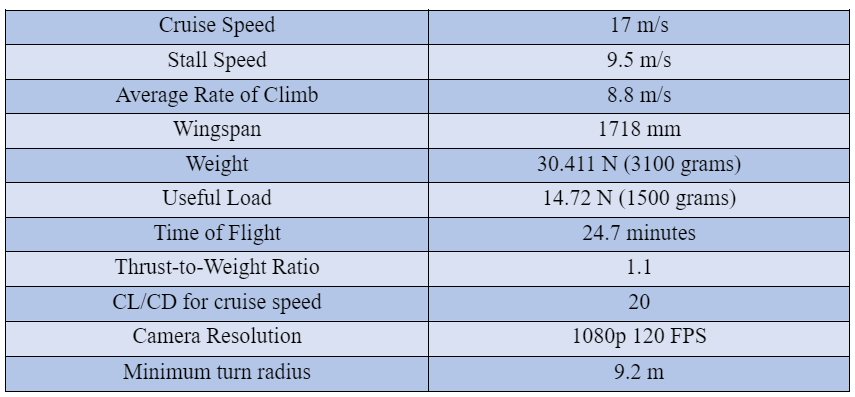
\includegraphics[width = .9\linewidth]{/table1.png}
 	\caption{Astrotech UAV's Performance Specifications}
        \label{fig:stall}
 \end{table}
\FloatBarrier


\justify
As a result of our calculations, Astrotech UAV’s takeoff weight is found 3100 grams, and the useful load is found 1500 grams, so we need 3100 grams of lift force to maintain a steady level flight. As a result, we find the cruise speed as 17 meters per second to provide this much lift force at low angle of attack values (0-2), in other words, to fly at a steady level. Moreover, the speed on the stall position, where the angle of attack rises beyond a specific point, then lift begins to decrease, is found at 9.5 meters per second by the formula:

\begin{align}
	V_{stall} = \sqrt{ \frac{2W}{\rho \cdot S C_{L max}}} 
\end{align}

\begin{figure}[ht]
 	\centering
 	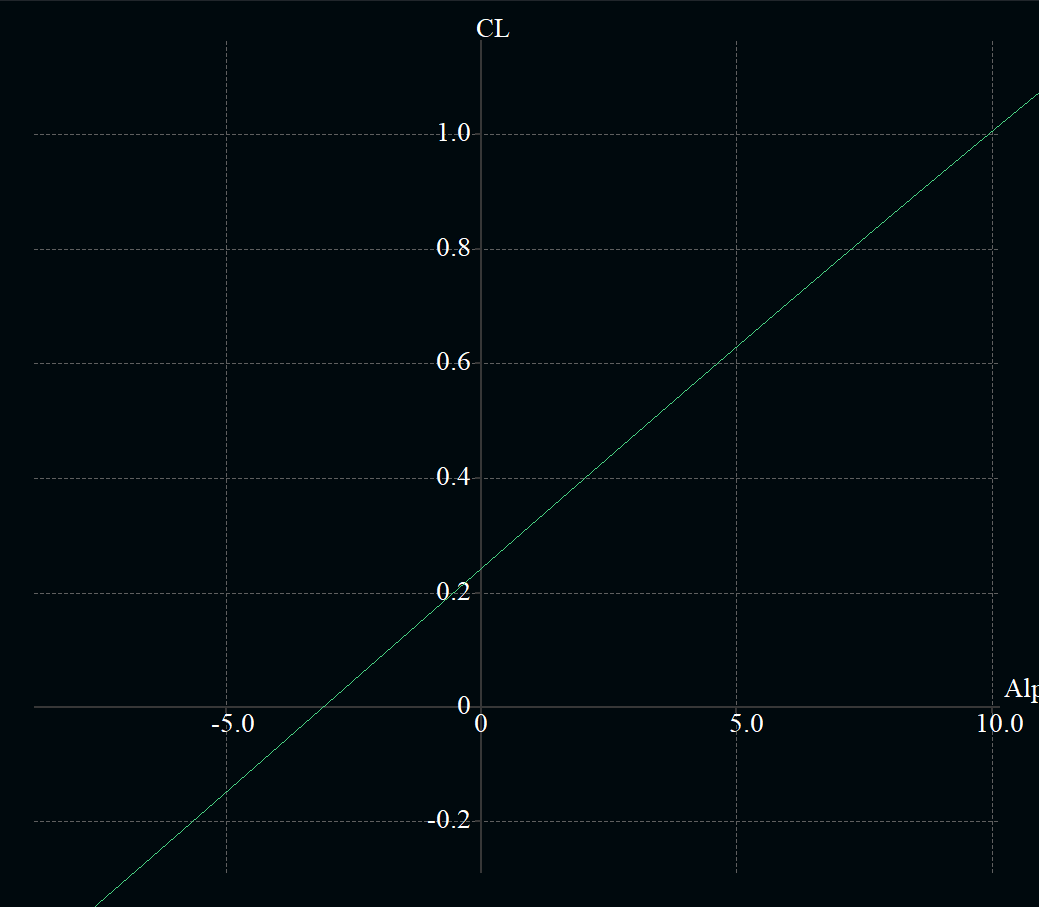
\includegraphics[width = .6\linewidth]{unnamed.png}
 	\caption{$c_L$ vs $\alpha$ Graph}
        \label{fig:stall}
 \end{figure}
\FloatBarrier
\justify
The flight time has been calculated as 24.7 minutes, and CL/CD ratio has been calculated as 20 for cruise speed. For detailed information, see 3.3 from the report.
\justify
The average rate of climb value of Astrotech UAV has been evaluated as 8.8 m/s by the formula:

\begin{align}
	R_{OC} = \frac{T \cdot V_\infty - D \cdot V_\infty}{W}
\end{align}

\justify
The weight of the aircraft is 30.411 Newton, thrust (T) equals 18.3 Newton, drag (D) equals 2.5 Newton, and the aircraft's speed is equal to 17 meters per second, that is, cruise speed. If the values are put in the equation, the rate of climb can be found as 8.8 meters per second.
\justify
Camera resolution is an important specification which affects the image quality and therefore influences our ability to detect or characterize objects of interest during tacking and detecting competitor UAVs. The decided camera module supports up to 120 fps for full HD resolution which is critical in any application involving fast motion.
\justify
It is expected that the companion computer can work at 30 FPS when selected image processing methods are used. NVIDIA Xavier NX Developer Kit has NVIDIA Volta architecture with 384 NVIDIA CUDA® cores, and 48 Tensor cores and these features are enough to satisfy our expectations. 
\justify
The minimum turn radius is found as 9.2 meters. While finding the minimum turn radius, the banking angle plays a vital role in finding the load factor (n) because the load factor is equal to $\frac{1}{\cos(\Phi)}$ where $\Phi$ is the banking angle. Moreover, if $\Phi$  approaches $\pi$/2, the load factor value goes to infinity and, therefore, $\frac{1}{n}$ becomes closer to 0. As a result, if we look at the minimum turn radius equation, which is $R_{min}=\frac{V^2_{stall}}{g \cdot \sqrt{1-\frac{1}{n^2}}}$ . Stall speed is 9.5 meters per second, g is the gravitational acceleration, which is equal to 9.81 meters per second square, and, if $\frac{1}{n}$ is equal to 0, the value inside the square root is the 1. As a result, the minimum radius turn value becomes 9.22 meters.


\section{ORGANIZATION SUMMARY}
\subsection{Team Organization}
\justify In this part of the report, the organizational chart of the team and the duties of the sub-teams are mentioned. Organizational chart of the METU Comet Astrotech Team is shown in Figure \ref{fig:stall}. As can be seen from the organization chart, the METU Comet Astrotech Team consists of three  sub-teams and finance \& logistics member. The detailed informations about the team members are as follows.

\begin{figure}[ht]
 	\centering
 	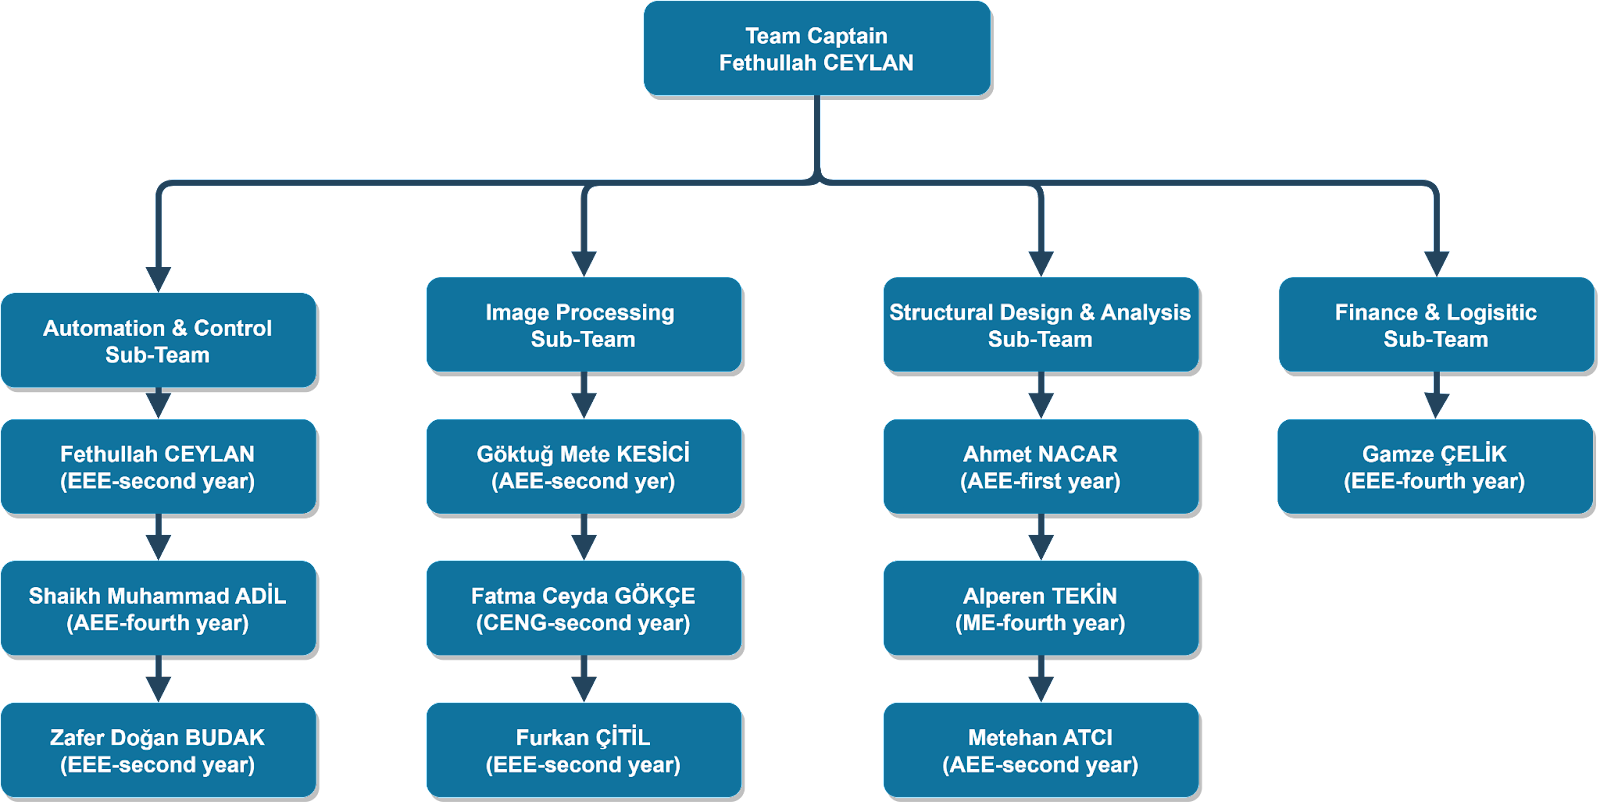
\includegraphics[width =\linewidth]{TeamChart.png}
 	\caption{Team Organization Chart}
        \label{fig:stall}
 \end{figure}
\FloatBarrier


\paragraph*{Fethullah Ceylan:} Sophomore electrical and electronics engineering student. He is the team captain responsible for team organization and time management. Also, he is working on path planning and virtual targets for testing.

\paragraph*{Shaikh Muhammad Adil:} Senior aerospace engineering student. He is working on virtual-based guidance and its ROS2-PX4 implementation.

\paragraph*{Zafer Doğan Budak:} Sophomore electrical and electronic engineering student. He is working on mission software development, integration and tests. 

\paragraph*{Göktuğ Mete Kesici:} Sophomore aerospace engineering student. He is working on the development of image processing software and its compatibility with the guidance algorithm.

\paragraph*{Furkan Çitil:} Sophomore electrical and electronics engineering student. He is working on the development of image processing software. Also, he helps the integration.

\paragraph*{Fatma Ceyda Gökçe:} Sophomore computer engineering student. She is working on ground control station. Also, she helps image processing software development.

\paragraph*{Ahmet Nacar:} Freshman aerospace engineering student. He is working on integration, manufacturing and testing. 

\paragraph*{Alperen Tekin:} Senior Mechanical engineering student. He is working on mechanical design and modelling of the UAV.

\paragraph*{Metehan Atcı:} Sophomore aerospace engineering student. He is working on the aerodynamic analysis of the UAV to achieve an understanding of its performance characteristics.

\paragraph*{Gamze Çelik:} Senior electrical and electronics engineering student. She is responsible for the budget management and sponsorships. 

\subsection{Timeline and Budget}
\paragraph*{Timeline:} The lines shown in blue show the content of the planned timeline announced in March. The works performed and the period in which they were carried out are shown in green. Worked parts of unfinished jobs are marked in yellow and the rest in red. The parts marked in red thus show the current plan as well.
\begin{table}[ht]
 	\centering
 	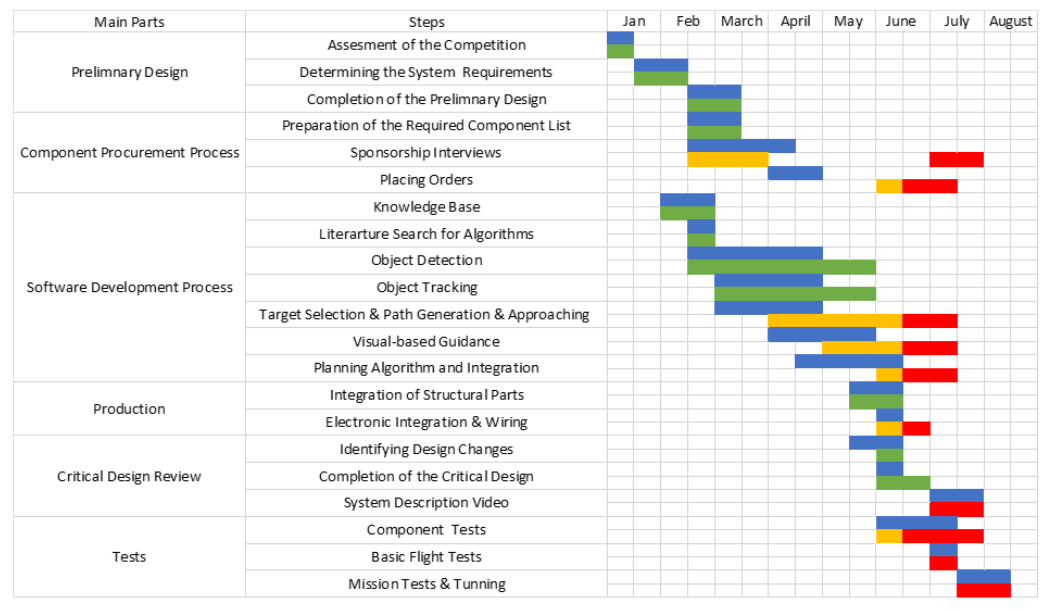
\includegraphics[width = \linewidth=.7]{/Timeline.png}
 	\caption{Timeline}
        \label{fig:timeline}
 \end{table}
\FloatBarrier
\clearpage 
\paragraph*{Budget:}The amount of money paid for the supplied products is shown in Figure 4 and marked in green. Products that are not yet supplied are marked in red and the current prices are added to the table. Estimations made in March are also included in the table. These all prices in Turkish Liras. The supply process of the products continues but to complete it competition support and additional sponsorship are required.
\begin{table}[ht]
 	\centering
 	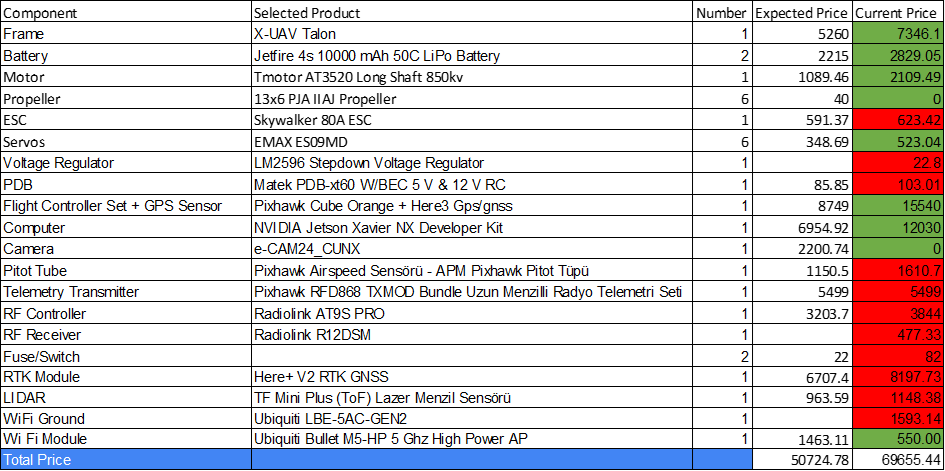
\includegraphics[width = \linewidth]{/budgetlist.png}
 	\caption{Budget List}
        \label{fig:budget}
 \end{table}
\FloatBarrier

\section{DETAILED DESIGN SUMMARY}
\subsection{Final System Architecture}
\justify
In this section, the final version of the system architecture, the brand / model information of the hardware to be used should be included. If there is a difference with the conceptual architecture, it should be stated and the reason should be explained.
\begin{figure}[ht]
 	\centering
 	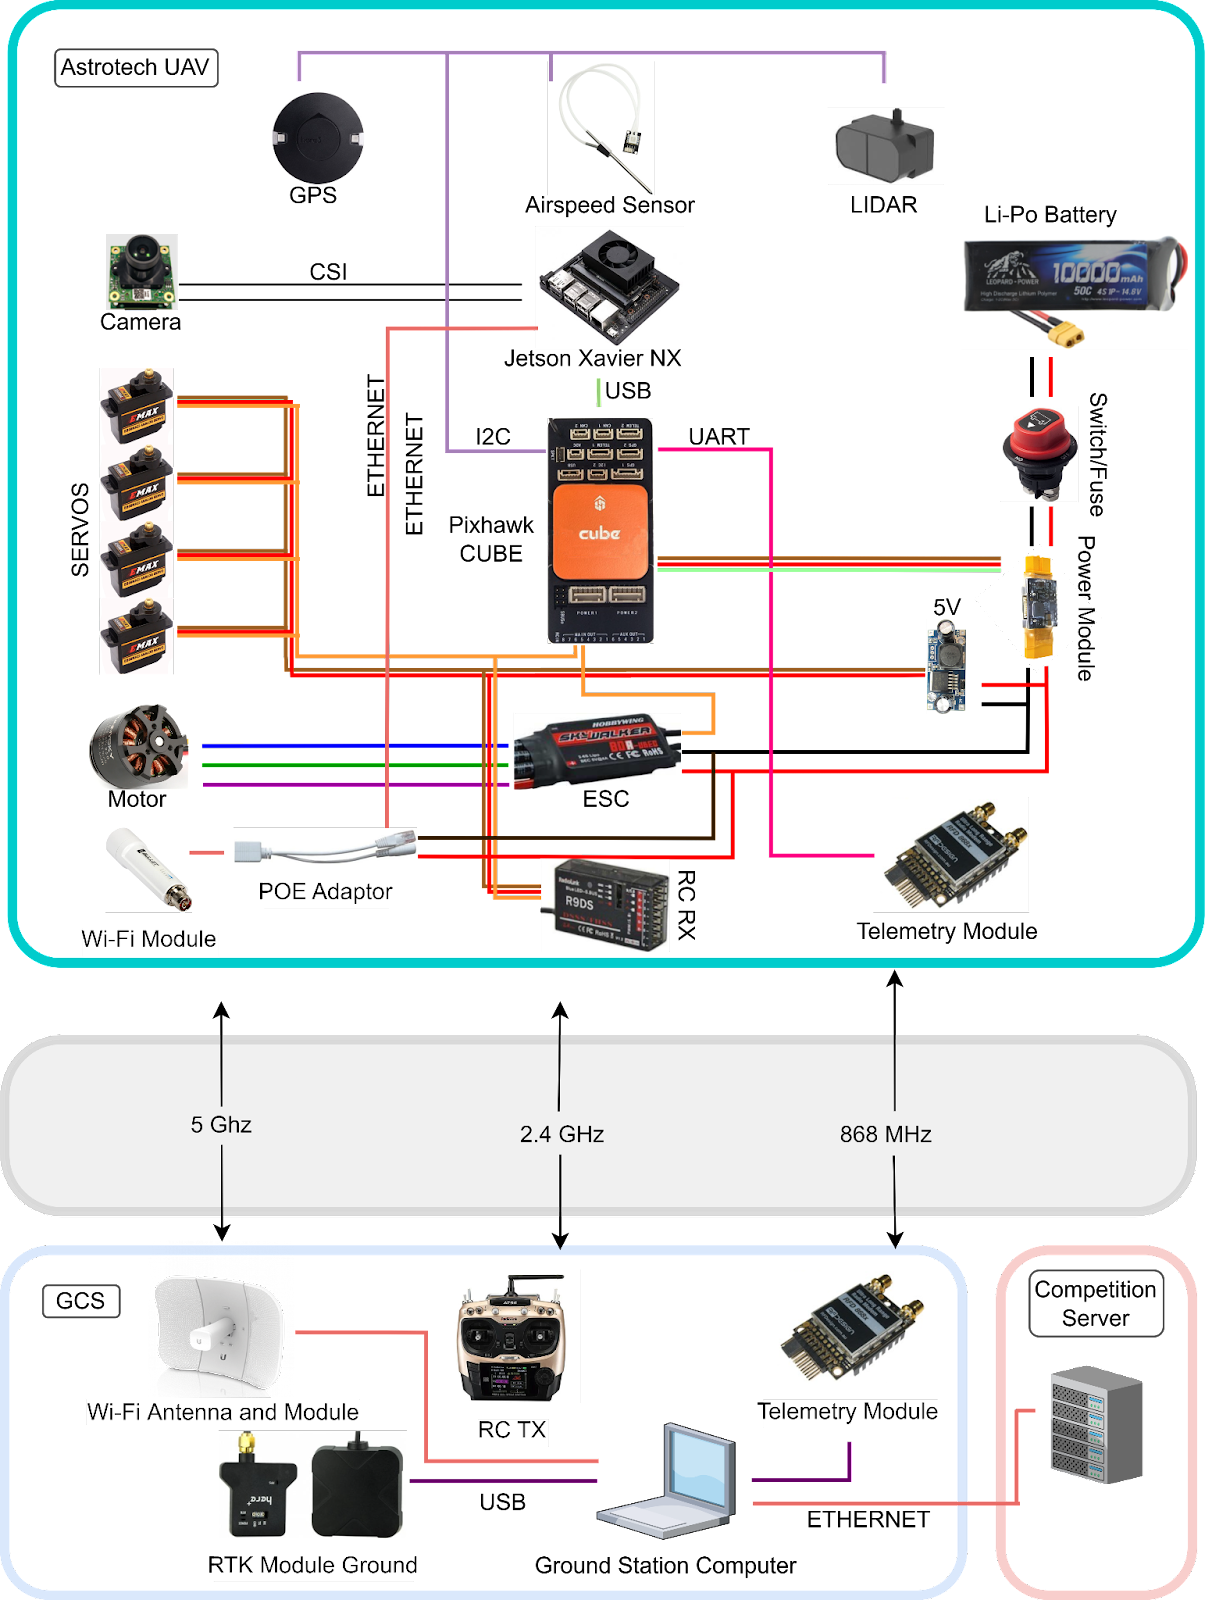
\includegraphics[width = \linewidth]{/sys_arc.png}
 	\caption{System Architecture}
        \label{fig:budget}
 \end{figure}
\FloatBarrier

\justify

\subsection{Subsystems Summary}
In this chapter; compliance of selected subsystems with vehicle requirements and selection criteria specified in the preliminary design report will be explained. If there is more than one option researched for the same duty, it should also be explained why the final product was chosen. 

\paragraph*{Flight Controller and GPS Sensor:} PX4 autopilot software is preferred to ensure the stability of the UAV during flight and to prepare the appropriate background for the autonomous mission software to be developed. Flight controllers compatible with this software were examined. Pixhawk Cube Orange is preferred because it has a lower error rate in IMU data than its competitors, is easily accessible, has detailed documentation and many sample projects. On the other hand, the reasons behind the selection of GPS sensor were RTK module compatibility, update rate, and low error rates. In this regard, it was decided that the Here+3 met our requirements, with 2.5 meters accuracy without using the RTK module. Also, when RTK module is used, the error value can be minimized up to 0.25 meters. 

\paragraph*{Companion Computer:} To obtain real-time performance, an onboard computing unit responsible for object detection and tracking as well as the guidance and target selection steps will be utilized. These computations would require relatively high computing power, thus; we preferred Nvidia Jetson Xavier NX, whose performance fulfills the requirements for relatively low cost. 

\paragraph*{Battery:} The electronics and the propulsion system of our aircraft will be powered by a Li-Po battery that has enough capacity for a flight time of 25 minutes. According to our calculations, a 4 cell Li-Po battery with a nominal voltage of 14.8V and a capacity of 10000mAh is enough for our aircraft when we also consider the safety margins. As we can see from the power consumption table below in part 3.3, which includes components with major power use, our battery with a capacity of approximately 150W/h is adequate to power our aircraft for more than enough time.

\paragraph*{Propulsion System and Servos:} For our UAV, we choose a motor-propeller pair that gives us the needed thrust to weight ratio of 1.1 as efficiently as possible.
\begin{table}[ht]
 	\centering
 	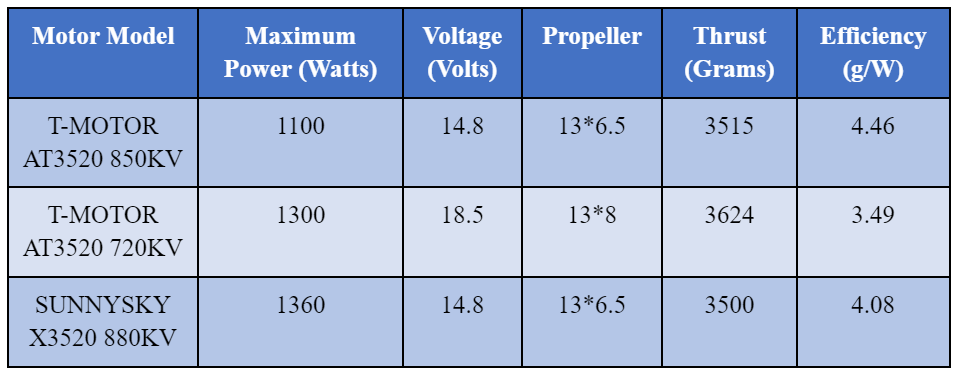
\includegraphics[width = .6\linewidth]{/motor_comp.png}
 	\caption{Comparison of several motors that are considered for the UAV}
        \label{fig:budget}
 \end{table}
\FloatBarrier
\justify 
On the table above, we can see the thrust values and efficiency of different motors. We choose the T-Motor AT3520 850KV Motor because of it sufficient thrust value and high efficiency. This motor is powerful enough to supply our aircraft with enough thrust for the entirety of the competition. For the manipulation of the control surfaces, we will use servo motors with enough torque to guide our aircraft. ES09MD Servo Motors are selected to be used. They are small, lightweight and have enough torque. They were also preferred because they have metal gears and can be driven digitally. To drive our motors, we will use an ESC with a maximum current of 80A with a built-in BEC. Hobbywing Skywalker 80A ESC is selected to be used as it can provide the necessary power to our system.

\paragraph*{Camera:} The features of the camera and its suitability for UAV  are mentioned. The selected camera is e-CAM24-CUNX, which is a Full HD MIPI CSI-2 global shutter camera. This camera is based on a 1/ 2.6” AR0234CS global shutter CMOS image sensor with a well-tuned ISP. Its global shutter capability along with 120fps frame rate helps to minimize frame to frame distortion and reduce the motion artifacts while capturing. Therefore, the UAV can obtain clear images of competitor UAVs while detecting and tracking. eCAM24-CUNX can be directly connected to the MIPI CSI-2 connector of the Nvidia Jetson platforms which are Jetson XavierTM NX/TX2 NX/Nano via Flex cable. Another advantage of the camera is that MISI CSI-2 is faster and has a reliable protocol to handle video from 1080p to 8k and has a higher net image bandwidth than USB. In addition, its DOFV is 133.9 and it meets the desired view for image processing algorithms.

\paragraph*{Pitot Tube:} To calculate the airspeed of our aircraft, we will use a pitot tube that is compatible with the flight controller. Ready To Sky Jmt PT60 Pitot Tube is found to be adequate for our system.

\paragraph*{RC Controller:} Radiolink AT10II and its transceiver RD12S have 12 channels for communication, 4km actual air range with 3ms transmission latency, which makes it suitable to use in Astrotech UAV. Also, another reason behind this selection is that it is more accessible to buy for the Metu Comet Astrotech team. 

\paragraph*{Telemetry Bundle:} To transmit telemetry data between UAV and ground station with high speeds and low loss rates, a telemetry bundle with such specifications is needed. With a 40 km air transmission range, RFD868x Telemetry Bundle is suitable for the needs of Astrotech UAV. 

\subsection{Aircraft Performance Summary:}
This section will demonstrate that the aircraft has propulsion that can remain in the air for the whole of a competition round.
\begin{figure}[ht]
 	\centering
 	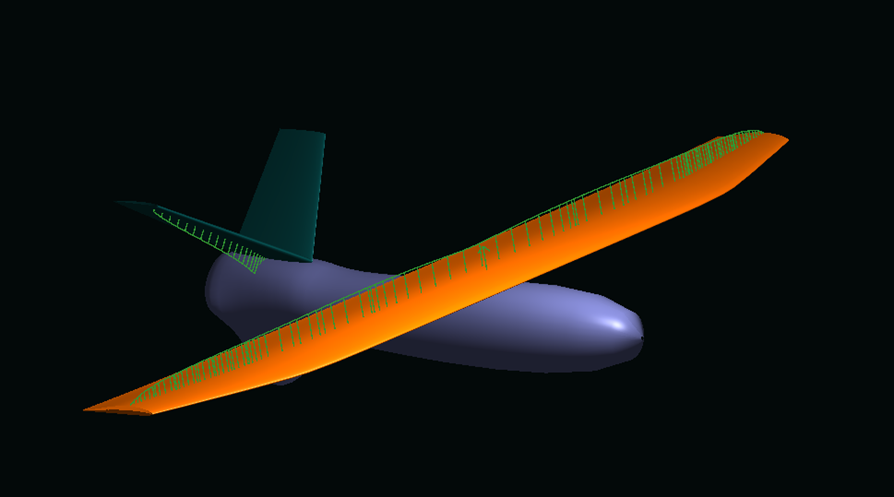
\includegraphics[width = .6\linewidth]{unnamed (4).png}
 	\caption{Comparison of several motors that are considered for the UAV}
        \label{fig:motorcmpr}
 \end{figure}
\FloatBarrier

\justify
Aerodynamic analysis of the Astrotech’s tail, wing, and body has been done using XFLR5, an aerodynamic analysis program (Figure 4.). As a result of the analysis, Lift coefficient vs. Drag Coefficient (CL/CD) vs. Alpha (α) is plotted, as shown in Figure 5. %TODO Figure X1 here

\begin{figure}[ht]
 	\centering
 	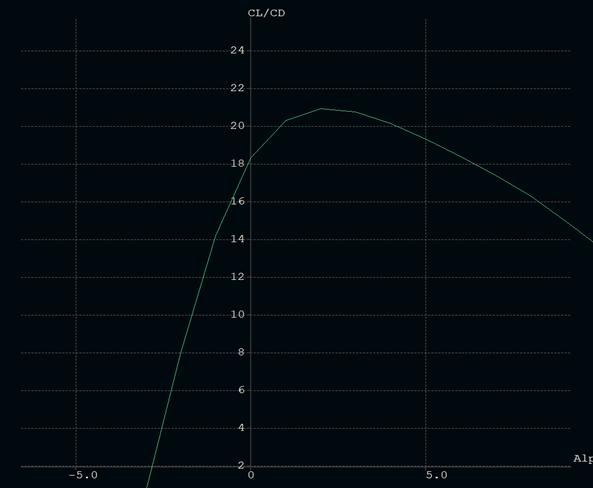
\includegraphics[width = .6\linewidth]{unnamed (5).png}
 	\caption{$c_L/c_D$ vs $\alpha$ Graph}
        \label{fig:motorcmpr}
 \end{figure}
\FloatBarrier
\justify
The CL/CD vs. Alpha graph represents the efficiency of the aircraft, and the more CL/CD means, the more efficient the aircraft is. Therefore, we want High CL/CD for less fuel consumption and, as a result, more time in flight. Moreover, in steady level flight which is the condition thrust (T) is equal to drag force (D) and Lift Force (L) is equal to the weight of the aircraft(W), we want higher CL/CD values. In the graph, the CL/CD ratio between the 0-2 angle of attack (desired steady level flight angle of attacks) is between 19-21.  Thus, CL/CD ratio is around 20 when the condition is steady. However, it is stated that CL/CD ratio can decrease after the external components takes its place on the aircraft \cite{Raymer2018}. Thus, after the external components such as servos are placed at the outer skeleton of the frame, we premeditate that this ratio can decrease up to 12. 

\clearpage
\justify
Moreover, in steady level flight, $T/D$ should be equal to $W/L \ \  (\frac{T}{D}=\frac{W}{L})$, and if we rearrange this equation, we can find the equation which plays a vital role in thrust calculations $\frac{T}{W}=\frac{D}{L}=\frac{C_D}{C_L}$. The weight of the aircraft is $30.411 Newton$ $(\frac{3100[g]9.81[m/s2]}{1000[g/kg]})$. The CL/CD ratio is 12 ($CD/CL$ ratio is $1/12$). If we put the values into the equation, we will find the required thrust for steady level flight as $2.53 Newton$ (260 grams). However, in a competition like the Fighting UAV, the competitor UAVs should be very aerobatic and maneuverable to accomplish the missions of the competition like dogfighting or kamikaze diving. During maneuvers, the engine has to generate more additional thrust. Therefore, 260 grams of thrust cannot be enough to succeed in the competition. Because of it, excess thrust should come into play through our thrust calculations. The average excess thrust has been calculated as $15.7 Newton$ (1600 grams). As a result, the required thrust force can be calculated as $18.3 Newton$ (1860 grams). Moreover, we can obtain 5m/s2 $(F_{net} (Excess Thrust) = m \times a )$ acceleration in x-direction with this excess thrust.       

\begin{align}
	Excess \ Thrust = Thrust \ Force \ - Drag \ Force
\end{align}

\paragraph*{Average Endurance:} The endurance can be changed by how much thrust is applied by the engine. For example, suppose the engine provides thrust just for the steady level flight. In that case, the endurance will be very high because the consumed power from the battery will be low. However, if it is allowed for \% 100 throttle, the endurance will be lower than the calculated endurance for steady level flight because the consumed power will be high. Therefore, it is needed to find an average value for endurance. Moreover, the thrust value we should look for is 1860 grams, and the corresponding consumed power value which can be found in the motor manufacturer’s datasheet is given in table \ref{fig:pwr_cns}. When all of the components are placed on the plane, they consume the power provided by the battery. Firstly, we find this consumed power, and after that, we should find the current by using the formula 4. Lastly, if we divide the ampere*hour of the battery by the current, we can reach the time that the frame can withstand in the air.

\begin{align}
	Power&= Voltage  \times Current \\
	 (P &= V \cdot I)\\
	\frac{10000 \ mAh}{1000 \ I } &= Time 
\end{align}

\begin{table}[ht]
 	\centering
 	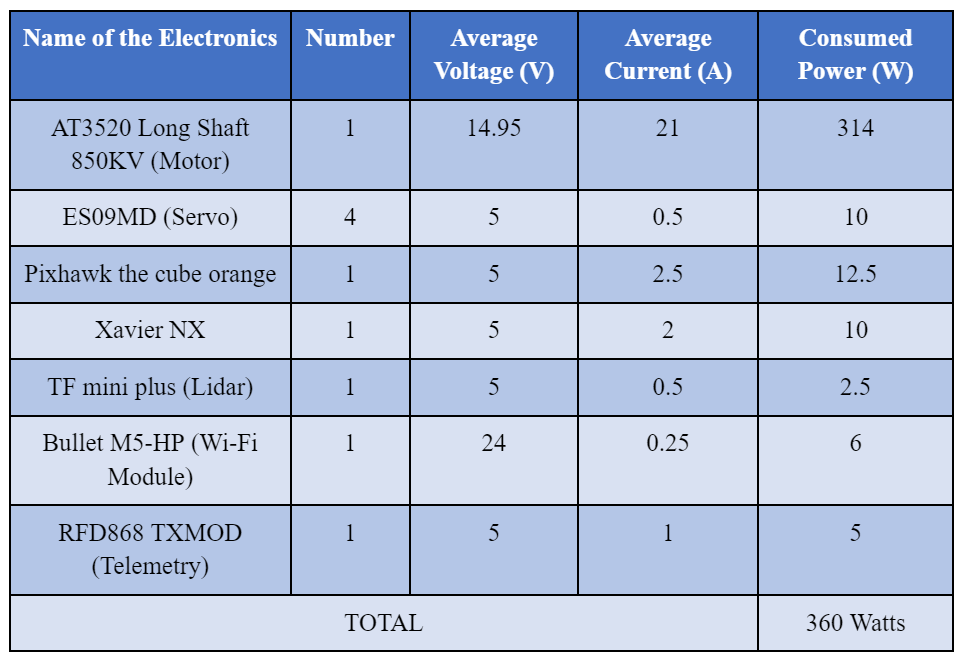
\includegraphics[width = .6\linewidth]{/power_cons.png}
 	\caption{Power Consumption of the Components}
        \label{fig:pwr_cns}
 \end{table}
\FloatBarrier
\justify
The consumed power of the components is found by using the formula 4. The total consumed power is seen as 360 Watts. Moreover, our battery’s voltage value is 14.8 Volts. If we put the voltage value of the battery with the total consumed power in the formula 4, we can find the average load current value of 24.32 Ampere. Furthermore, we know that the battery has 10000 mAh and the average load current is 24.32 Ampere. As a result, we can find the time using the formula 6. The average endurance is found as 0.411 hours, equal to 24.7 minutes. Considering that the Fighting UAV competition will last 15 minutes, it can be seen that the average endurance is 9.7 minutes, more than the required time. Thus, our project is suitable for competition requirements.  Moreover, the test procedure cannot be done yet due to delayed financial support from Teknofest.
%Todo Figure here

\subsection{3D Design of Aircraft}

Astrotech UAV is the Eagle Talon model aircraft produced by X-UAV company and the 3D design of this model aircraft is not available on the Internet, so it has been designed using the CATIA and ANSYS Spaceclaim. In addition, the assembly process and technical drawing of the components has been done with the ANSYS Spaceclaim. While performing the structural integration of the Astrotech UAV, these integrations are made with considering the dimensions and weights of the avionics used, their distance from the center of gravity of the UAV and minimum cabling. Some components which need to be taken out or taken in often, such as batteries, or have too much cable connections must be placed easily accessible positions where are chosen close to the upper cover part. Power and data lines of electronics telemetry of high current power cables, for example, in such a way that they affect each other the least. It should also be considered that it is placed in places far from each other so that it does not affect the signal. has been kept. The technical drawing and CAD drawing of the Astrotech UAV is shown in Figure 6 and Figure 7, the dimensions in mm are shown in Figure 7, and the positioning of the avionics placed in it are shown in Figure 8 and Figure 9. Wiring is not included in this positioning.
\begin{figure}[ht]
 	\centering
 	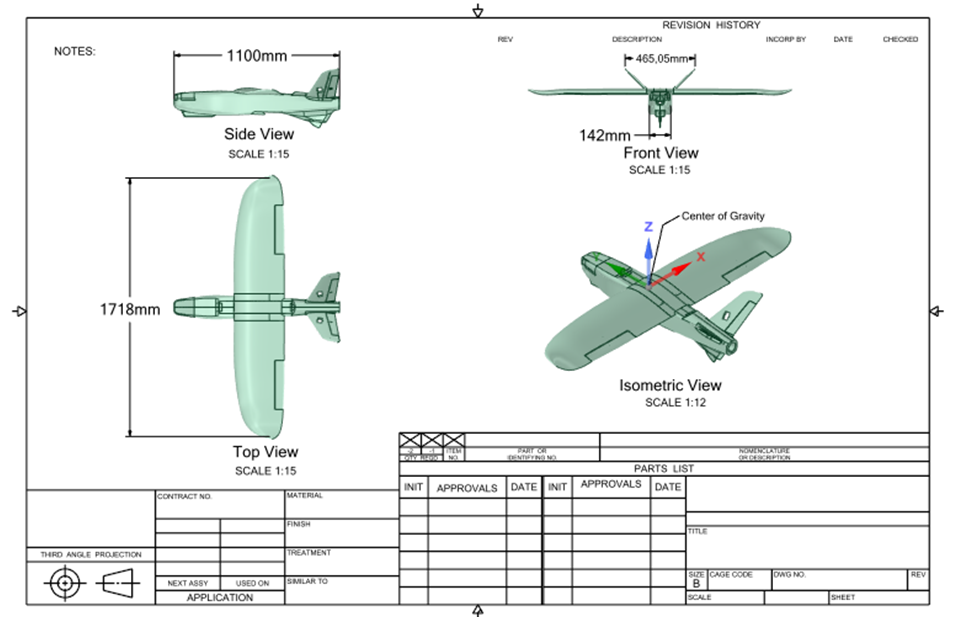
\includegraphics[width = \linewidth]{/unnamed (6).png}
 	\caption{Astrotech UAV Technical Drawing}
        \label{fig:Tech_izo}
 \end{figure}
\FloatBarrier

\begin{figure}
     \centering
     \begin{subfigure}[b]{0.4\textwidth}
         \centering
         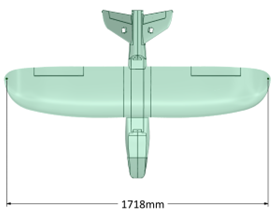
\includegraphics[width=\textwidth]{unnamed (7).png}
       \end{subfigure}
     \hfill
     \begin{subfigure}[b]{0.5\textwidth}
         \centering
         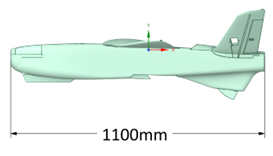
\includegraphics[width=\textwidth]{unnamed (9).png}
     \end{subfigure}
     \hfill
     \begin{subfigure}[b]{0.8\textwidth}
         \centering
         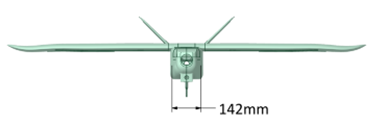
\includegraphics[width=\textwidth]{unnamed (8).png}
     \end{subfigure}
     \caption{Astrotech UAV Top, Front and Side View}
    \label{fig:three graphs}
\end{figure}
\FloatBarrier
\justify
The location of components is given in the Figure 8. The points taken into consideration while making this distribution are the center of gravity and the comfort it offers to the user. There is enough space in the front part of Astrotech UAV for the battery. In this way, adjustments can be made to keep the center of gravity at the desired point.

\begin{figure}[ht]
 	\centering
 	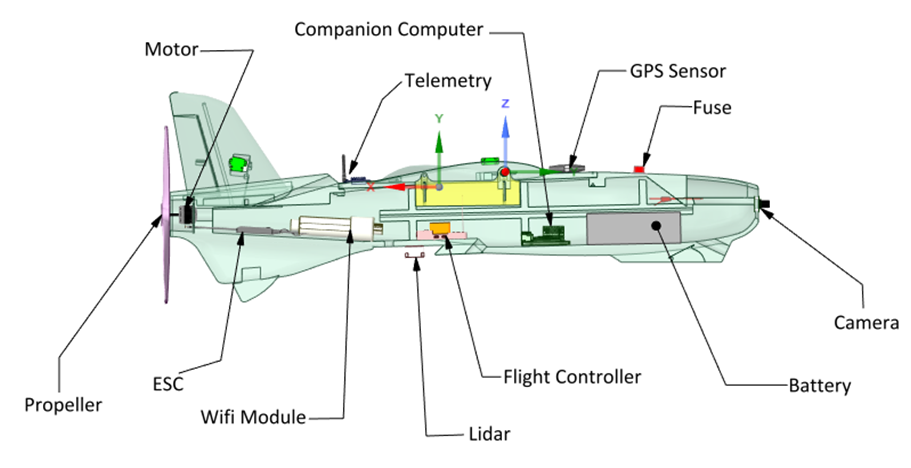
\includegraphics[width = .75\linewidth]{/unnamed (11).png}
 	\caption{Astrotech UAV Components Assembly Side View}
        \label{fig:assembly_side}
 \end{figure}
\FloatBarrier
\justify
The top view of Astrotech UAV is given below. In the following figure the location of pitot tube and servos where is placed in wing and tail is given below. In the following figure the one part of symmetry can be seen. Also, there are servos in the other side of Astrotech UAV.

\begin{figure}[ht]
 	\centering
 	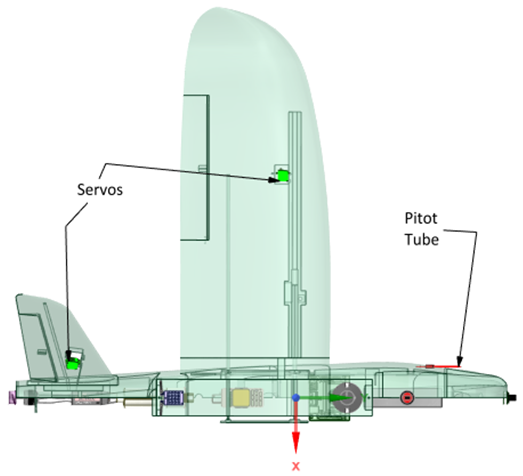
\includegraphics[width = .6\linewidth]{/unnamed (12).png}
 	\caption{Astrotech UAV Components Assembly Top View}
        \label{fig:assembly_top}
 \end{figure}
\FloatBarrier



\subsection{Aircraft Weight Distrubution}

The location of the center of gravity is one of the most important factors affecting the flight characteristics of the UAV. In addition to a stable flight of our aircraft, high maneuverability is required for the missions. According to the information provided by the company which produce this frame, when only the frame is considered, the center of gravity is 75mm behind the leading edge of the wing. As a result of both the information provided by the company and the analyzes made, the center of gravity was adjusted according to this point. The layout of the components is planned to determine the center of gravity at this point. Detailed weight, moment and center of weight calculation are given in detail in the Table 6 below. The center of gravity can be seen in the following figure \ref{fig:CG}.

\begin{figure}[ht]
 	\centering
 	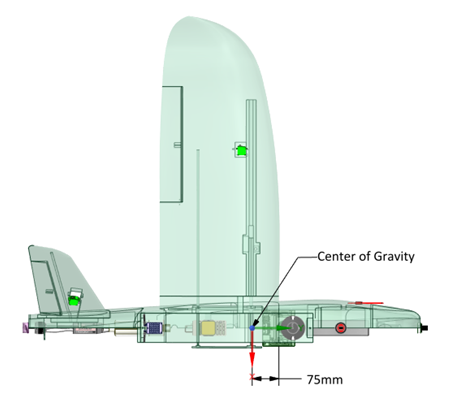
\includegraphics[width = .5\linewidth]{/unnamed (10).png}
 	\caption{Astrotech UAV Center of Gravity}
        \label{fig:CG}
 \end{figure}
\FloatBarrier
%\ref{fig:CG} bu

\justify
The calculation is given Table 6 below. The moment according to x and y axis is calculated. According to x-axis the moment is 0 (gr*mm). According to y-axis the moment is 0,8 (gr*mm) which is equal to 0,8*10-6 (kg*m). This result is negligible. 

\begin{table}[ht]
 	\centering
 	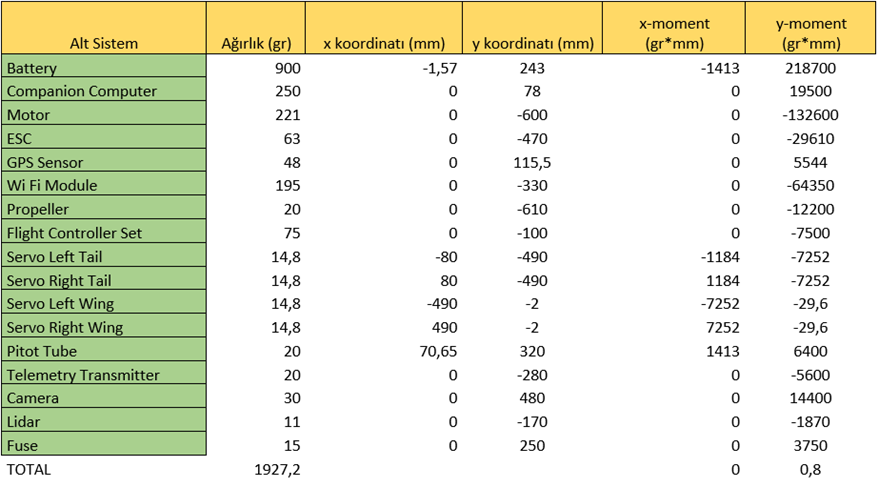
\includegraphics[width = .7\linewidth]{/unnamed (13).png}
 	\caption{Astrotech UAV Moment Calculation}
        \label{fig:moment}
 \end{table}
\FloatBarrier


\section{AUTONOMOUS MISSIONS}
There are two missions to be performed in the competition and it was decided to gather these missions within a single software architecture. When the UAV is initialized and the flight mode is changed to Offboard mode, the mission code will start to be executed. The overall design of the flow of autonomous mission code is shown at Figure \ref{fig:flow}.  Also at Figure \ref{fig:flow}, the part described as “Missions” is shown explicitly. 

\begin{figure}[ht]
 	\centering
 	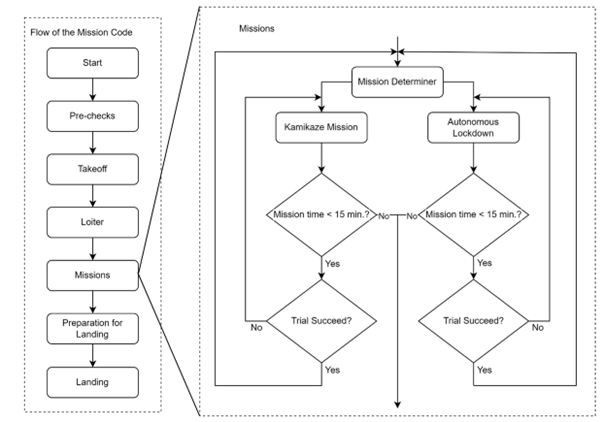
\includegraphics[width = .6\linewidth]{/flowmissioncode.png}
 	\caption{Flow of the mission code}
        \label{fig:flow}
 \end{figure}
\FloatBarrier
\justify
The detailed information about these missions is given under 4.1 Autonomous Lockdown and  4.2. Kamikaze Mission.

\subsection{Autonomous Lockdown}
The main strategy in the autonomous lockdown mission is to select the ideal target, approach the target from behind and lock it, and keep the target within the camera view for 4 seconds with vision-based guidance. The steps and related explanations required for this strategy are given under this heading.
\subsubsection{Path Planning, Cost Evaluation, and Target Selection}

\begin{figure}[ht]
 	\centering
 	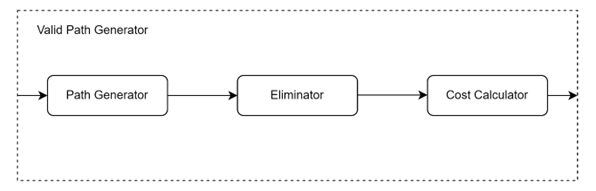
\includegraphics[width = .6\linewidth]{/validpathgenerator.png}
 	\caption{Structure of valid path generator}
        \label{fig:moment}
 \end{figure}
\FloatBarrier

\justify For the autonomous locking, firstly the target must be approached from the appropriate angle and distance so that the next stage of the mission, vision-based guidance, can be performed. There are two requirements for this approach, which are target detection and path planning. While the ideal target for any moment during the competition is variable, there is also the possibility that some UAVs will be easier targets compared to other UAVs during the competition. However, it would be more reasonable to start developing the basis of the target selection algorithm for UAVs, considering all of them are equal. Afterwards, it is possible to make some additions to this basic algorithm according to the weaknesses of the UAVs. Our motivation behind this choice is to keep the development process as less complicated as possible.
\justify In the following chapters, one of the implementations of Dubin's Path Generation Algorithm is used for the development, rearrangements on the path generation algorithm for dynamic targets, and the criteria for choosing among the generated paths are explained. Finally, it is mentioned how our algorithm can be modified for more vulnerable targets.

\paragraph{Dubin’s Path Generation Algorithm}
In order for the UAV to approach the target correctly, a path suitable for the flight characteristics must be generated between the current location and the target location. Dubin's Path is a method used to draw 2D roads with similar motivations, especially in non-holonomic land vehicles \cite{Reeds1990OPTIMALPF}. However, this method is not sufficient for our case, as it is since it cannot be applied to aircraft moving in a 3D environment directly. Although it is not complete for our use case it is a good starting point since our plane is also a non-holonomic vehicle.
\begin{figure}[ht]
 	\centering
 	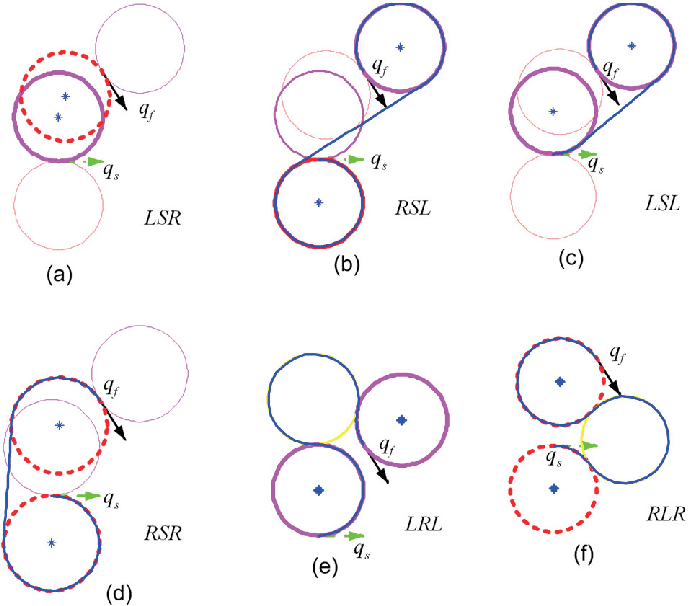
\includegraphics[width = .75\linewidth]{/dubins2d.png}
 	\caption{Examples of 2D Dubin’s Paths having different shapes \cite{inproceedings}}
        \label{fig:moment}
 \end{figure}
\FloatBarrier

\justify
To generate such paths in 3D environments from a vector to vector with constraints such as turning and climbing, an improved version of Dubins path from 2D to 3D, also named Dubins Airplane, is proposed in the following paper\cite{s20020547}. While this work is the reference point for the implementation by our team, it does not exactly match the work of Owen and others. Along with this implementation, which was developed over the vector field methodology, Demirdal's study is also used as a reference in the developed software \cite{Tolga2022}. In his study, It is observed that the 2D Dubin’s Path on the x-y plane projected on a plane according to the maximum pitch rate, and in where the circular motions occur piecewise interpolation was used. Also, this implementation runs fast enough to calculate all possible paths for each rival UAV. In Figure \ref{fig:Dpath1} and \ref{fig:Dpath2} two examples of paths generated by this implementation is shown.

\begin{figure}
\centering
\begin{subfigure}{.5\linewidth}
  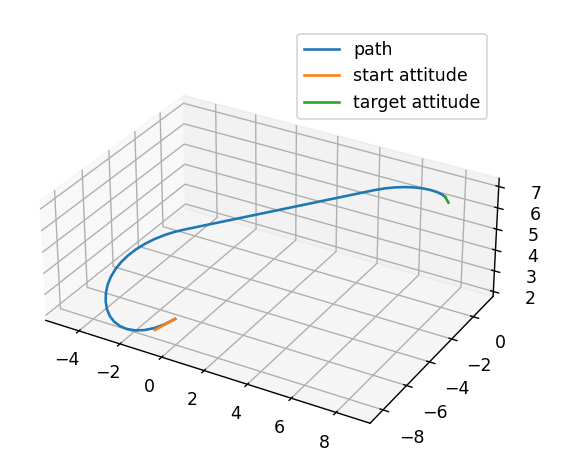
\includegraphics[width=.75\linewidth]{dubins3d_1.png}
  \caption{RSR configuration}
  \label{fig:Dpath1}
\end{subfigure}%
\begin{subfigure}{.5\linewidth}
  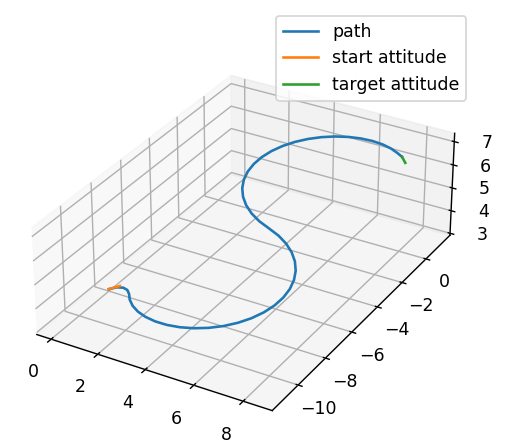
\includegraphics[width=.75\linewidth]{dubins3d_2.png}
  \caption{RLR configuration}
  \label{fig:Dpath2}
\end{subfigure}
\caption{3D path examples}
\label{fig:test}
\end{figure}
\FloatBarrier
\justify
In an environment where data flow is limited and the targets are in motion, this study is necessary but not sufficient as a solution. Because, in our case, there is uncertainty about the target location and heading which are the inputs in these algorithms. Also, collision with the target is undesirable. In the following chapter, these problems are examined and further discussed.

\paragraph{Rearrangements on Path Planning for Dynamic Targets}
\justify It is necessary to determine how much and in what direction the rival UAVs have moved and will be moving until the next data packet arrives. If this estimation is made for longer time intervals, the accuracy of the prediction will decrease. If the time between two data packages is taken as one second, even the position information of the rival UAVs in the last few data packages will be sufficient for this estimation. But beyond this estimation, towards the end of this approach phase, when trying to determine the location of the target UAV, it is difficult to find a close answer. There are many factors that increase this uncertainty, and it is very difficult to take all of these factors into account. Therefore, the estimation of the future location needs to be limited at some point.
\justify Making an estimation of the position after a determined time by applying curve fit on the position and velocity information was considered as a solution. How long after the estimation meets the requirements will be determined as a result of the simulation and test studies. In particular, tests with virtual targets described in 8.2 Flight Tests and Flight Checklist play an important role in this regard. 
\justify Another adjustment to be made in path generation is that all paths that are normally eliminated during generation are taken into account. These paths are eliminated because they do not have the ideal configuration (e.g. RSL, LRL) for the current situation. However, different criteria have been defined in the designed algorithms regarding what the ideal configuration is, and this necessitates the evaluation of all options.
\paragraph{Cost Evaluation and Criteria}
\justify After the generation of paths it is necessary to find the ones which are valid according to our criteria. Also, the cost of the paths must be calculated to choose best one. The modified version of the implemented dubins path will give costs for different paths. These costs will be calculated according to the parameters of the length of the path calculated. After that the paths which are going out of the mission area are eliminated. To determine if a path is in the mission area or not, the 3D path will be projected into X-Y(ground-plane) and then it will be simply checked whether the path is in the margins of the mission area. 
\justify Another important criteria is related to the target. Changing the target UAV repeadetly even without trying to get close to it is an unwanted situation. Thus, the paths belonging to followed target are more likely to be chosen. Also, if locking is succesfully completed, the paths belonging to the last target will not be taken into account. 
\paragraph{Biased Target Selection}
For the biased target selection part the costs and possible paths for UAVs will be firstly evaluated like mentioned in the previous part. This evaluation will be sufficient for basic selection of targets. However because of the fact that some UAVs will be easier targets than other regarding their flight characteristics and total locks. A bias can be added for the cost evaluation of every target. Then according to the determined costs a path can be selected.

\subsubsection{Approaching the Selected Target}
At this point a path is selected for a target however because of the non-holonomic movement characteristics of the aircraft it will not be possible to directly follow the desired path. For that a pursuit algorithm will be used. A pursuit algorithm function here is to make the vehicle regain its path and maintain it according to the desired path in an efficient way. 
There are two different path followings algorithms inspected for the our use case, namely “Pure Pursuit” and “Vector Pursuit”. Since vector pursuit is more complicated and hard to implement, vector pursuit is prefered. Also, since pure pursuit is used to determine the points in space when sending the setpoint commands which enables smooth responses thanks to L1 controller, there is not much reason to use such a complicated algorithm.  
When determining the parameters like look ahead distance, the observations obtained via tests and simulations will be used.  
\subsubsection{Image Processing} 
\justify In this part, image processing algorithms will be discussed. For real time guidance, image processing algorithms are required so that the rival UAV would be located on the onboard camera with respect to our UAV. Image processing consists of two parts, object detection and object tracking respectively. Once the rival UAV is detected and localized with an object detection algorithm, its output is fed into the object tracking algorithm. Then, the object tracking algorithm will track the rival UAV until N frame passes, which can be seen from the figure below. Benchmark tests \cite{isaac2021unmanned,fu2020correlation,nepal2022comparing,redmon2016you,redmon2018yolov3,zhang2018fast,li2020agricultural} of state of art algorithms are investigated during the literature research to find most appropriate algorithms for our case.
\justify The composition of detection and tracking algorithms allows us to perform image processing task with higher speed on an onboard computer, which is essential for an agile system, because tracking algorithms mostly outperform detection algorithms in terms of speed. In the competition, these image processing algorithms will run on an onboard computer because real-time control with low latency can be achieved and a more agile system can be obtained in this way. Also, a computer on a ground control station is considered to process the image, but this option comes with delays during data transfer between GCS and the UAV. Therefore, image processing algorithms that can run on onboard embedded computers are researched. 

\begin{figure}[ht]
 	\centering
 	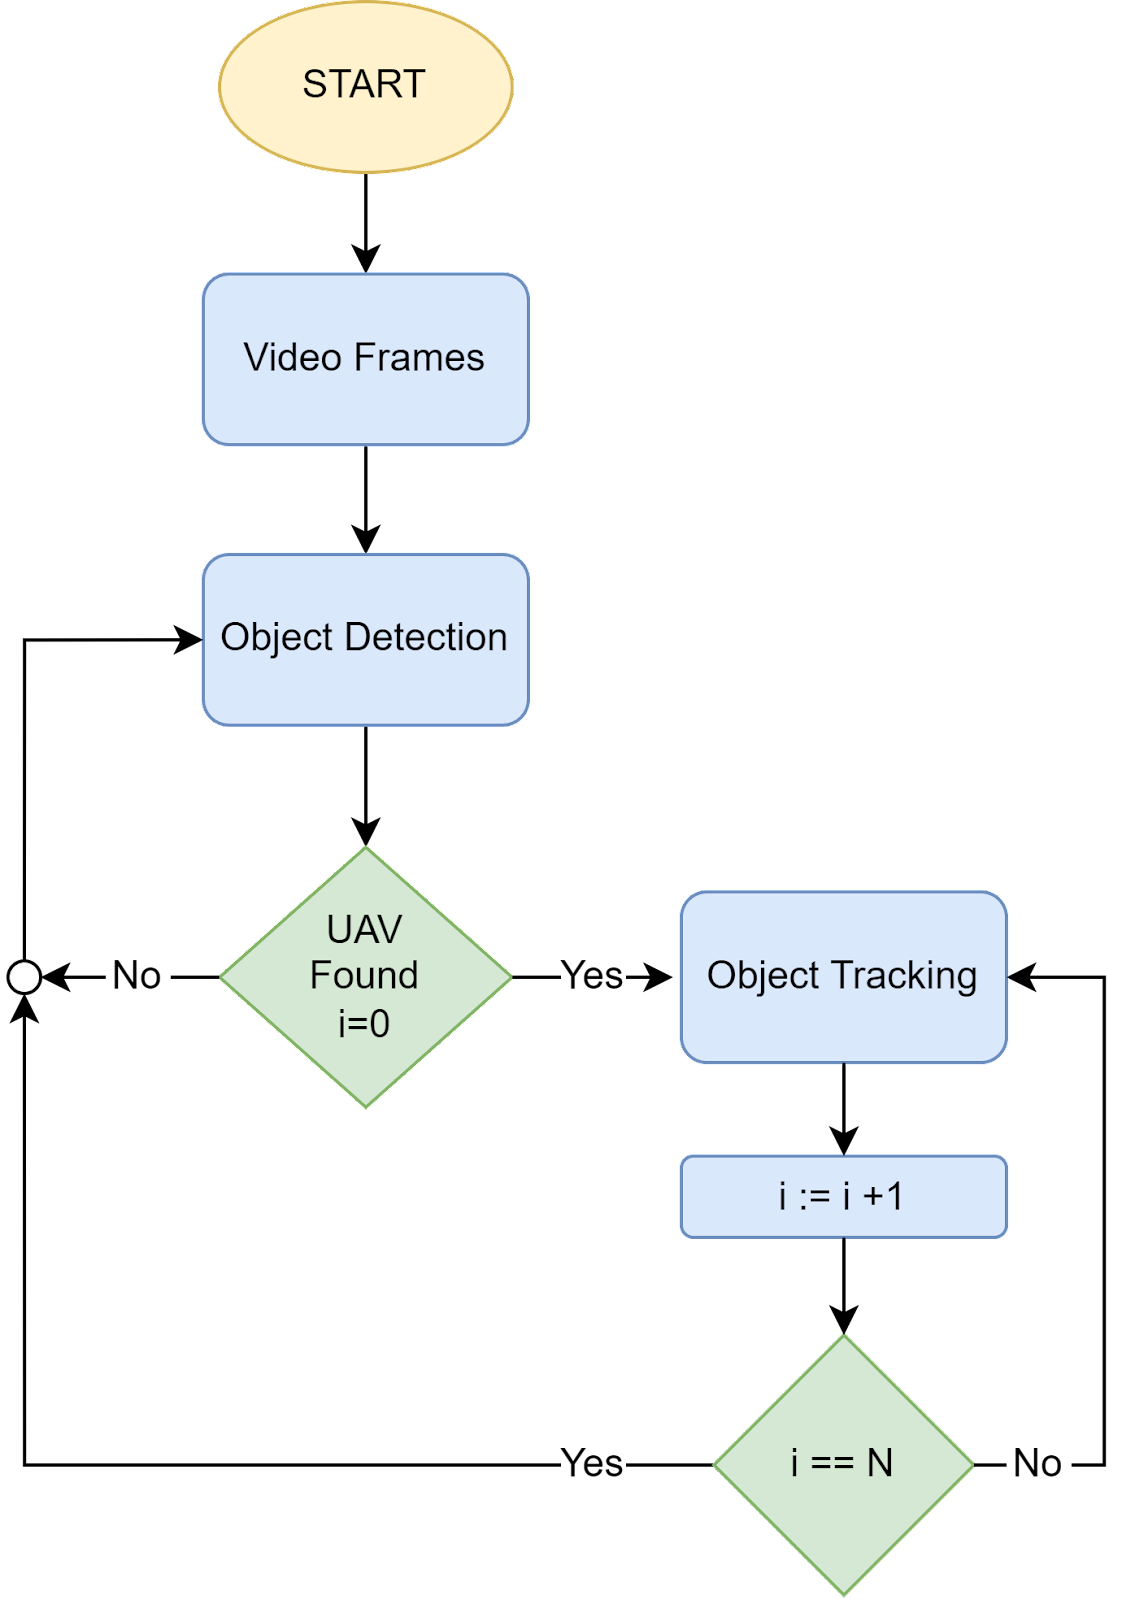
\includegraphics[width = .5\linewidth]{/ip_flow.png}
 	\caption{Flowchart of Image Processing Algorithm}
        \label{fig:moment}
 \end{figure}
\FloatBarrier

\paragraph{Object Detection}
\justify Different approaches are used for object detection, and we examined them into two major parts. These are two-stage detectors, such as the RCNN family, and one-stage detectors, such as SSD, YOLO, and RetinaNet. The two-staged detectors yield relatively high accuracy, yet they are not suitable for real time applications, hence; not applicable for our purpose \cite{redmon2018yolov3,zhang2018fast, li2020agricultural}. On the other hand, the one-stage detectors are slightly less accurate, but they offer better FPS values \cite{zhang2018fast}, and the majority of them can be used for real-time applications, except RetinaNet \cite{zhang2018fast}.
\justify Examining the literature and benchmarks, it is realized that YOLO outperforms the majority of the other algorithms, and it is best fit for the use of this competition.
\begin{table}[]


\resizebox{\textwidth}{!}{\begin{tabular}{llll}
\hline
Reference                 & Dataset                                                        & Algorithm                                                            & Conclusions                                                         \\ \hline
Li et al., 2021 \cite{li2020agricultural}  & Remote sensing images collected from GF-1 and GF-2 satellites. & \begin{tabular}[c]{@{}l@{}}Faster R-CNN\\ YOLO v3\\ SSD\end{tabular} & YOLOv3 has higher mAP and FPS than SSD and Faster R-CNN algorithms. \\ \hline
Rahman et al.,  \cite{rahman2021autonomous}  & Custom Electrical dataset                                      & \begin{tabular}[c]{@{}l@{}}YOLOv4\\ YOLOv5l\end{tabular}             & YOLOv4 has higher mAP compared to YOLOv5l algorithms                \\ \hline
Long et al., \cite{long2020pp}    & MS COCO dataset                                                & \begin{tabular}[c]{@{}l@{}}YOLOv3\\ YOLOv4\end{tabular}              & YOLOv4 has higher mAP compared to YOLOv3                            \\ \hline
Kim et al., 202\cite{kim2020comparison} & Korea expressway dataset                                       & \begin{tabular}[c]{@{}l@{}}YOLOv4\\ SSD\\ Faster R-CNN\end{tabular}  & YOLOv4 has higher accuracy SSD has higher detection speed           \\ \hline
\end{tabular}}
\caption{Benchmarking of the state of art Algorithms \cite{redmon2016you}}
\end{table}
\justify One of the major drawbacks of the YOLO algorithm is that on Xavier NX, which would be used as the companion computer, the YOLOv3, YOLOv4, and YOLOv5 operate between 5-7.5 FPS approximately \cite{redmon2016you}. The real-time applications require at least 20 FPS, and hence; we settled on the use of either YOLOv3-tiny or YOLOv4-tiny. However, it is important to note that the YOLOv3 algorithm has some major drawbacks, one of which is relatively poor performance for medium and large objects \cite{zhang2018fast}. Another problem of YOLOv3 is that it struggles to align the bounding box with the objects with high accuracy \cite{zhang2018fast}, which can be a problem for our method that heavily depends on the object tracking algorithm. It is presumed that these problems might also be inherited by YOLOv3-tiny, so we decided to use YOLOv4-tiny for object detection. The training is done on Google Colab to leverage high performance GPUs and decrease the required time to train the network.  Also, we anticipate that the detection algorithm would work real-time using the OpenCV library, yet in case this approach does not provide real-time performance, the TensorRT library would be utilized to improve the inference time of the detection process.

\subparagraph*{Architecture of YOLOv4-tiny}

\justify YOLOv4-tiny is mainly composed of the backbone, neck and head. The backbone is responsible for extracting useful information in different sizes from raw images, and in this particular algorithm, it is achieved by using CSPDarknet53-tiny. After extracting the useful information the neck structure takes them as inputs, and by combining the feature maps obtained at different stages, it returns the information which is later on used by the head structure. This process is mainly done to construct a rich, multi-scale feature pyramid by using a top-down pathway and lateral connections, which provides multiscale predictions \cite{bertinetto2016fully}, and YOLOv4-tiny adopts Feature Pyramid Network (FPN) as neck structure. Finally, the head structure accepts the outputs of the neck as inputs, and it returns a matrix that contains the coordinates of the bounding boxes and the prediction scores for each class. In YOLOv4-tiny, YOLO heads are used for the head structure. 
\begin{figure}[ht]
\centering
 	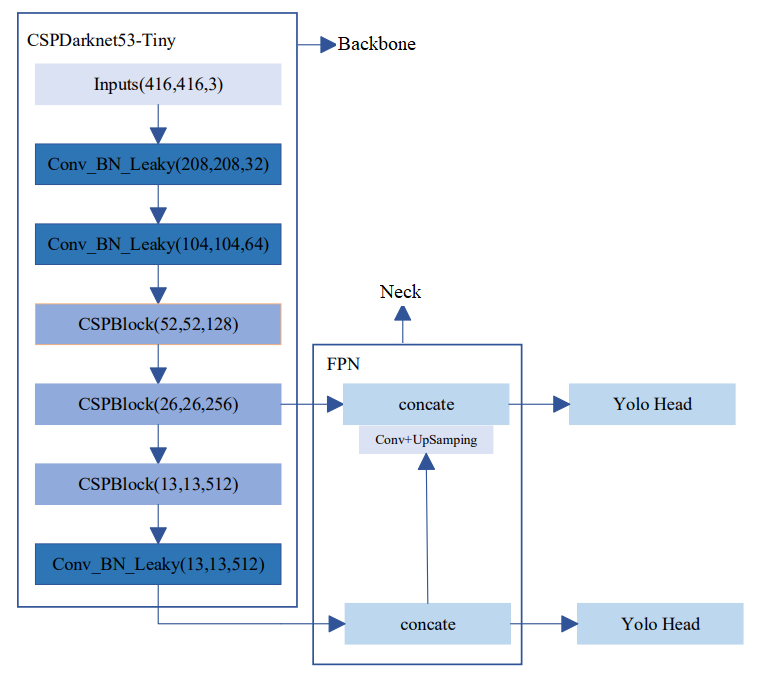
\includegraphics[width = .6\linewidth]{ip_blockdiagram.png}
 	\caption{Flowchart of Image Processing Test \cite{lin2017focal}}
    \label{fig:moment}
\end{figure}

\FloatBarrier
\justify Some additional methods, such as non-max suppression and anchor boxes are also applied to improve the performance even further. The use of non-max suppression enables us to avoid overly crowded bounding boxes for the same object. The idea is that if the intersection of the bounding boxes exceeds a threshold value, all the bounding boxes but the one with the highest confidence score are suppressed. The other method, anchor boxes, make it possible for the predictions to be done by taking into consideration the aspect ratios of the objects. Thus, for each grid cell, several objects having different aspect ratios can be detected with the help of the anchor box method.


\paragraph{Object Tracking}
\justify In the second part of image processing algorithm, detected object, rival UAV, will be tracked with an object tracking algorithm. The main objective of the object tracking algorithm is to predicit the state of the object based on the its initial state. Object tracking algorithms are categorized into two groups: single object tracking and multiple object tracking. In this competition, Although there will be  more than one rival UAV in the air simultaneously, we will be only focusing on a single UAV with image processing, so single object tracking algorithms address the object tracking problem for us. There exists various single object tracking algorithm in the literature.  These algorithms are categorized in the figure below:
\begin{figure}[ht]
 	\centering
 	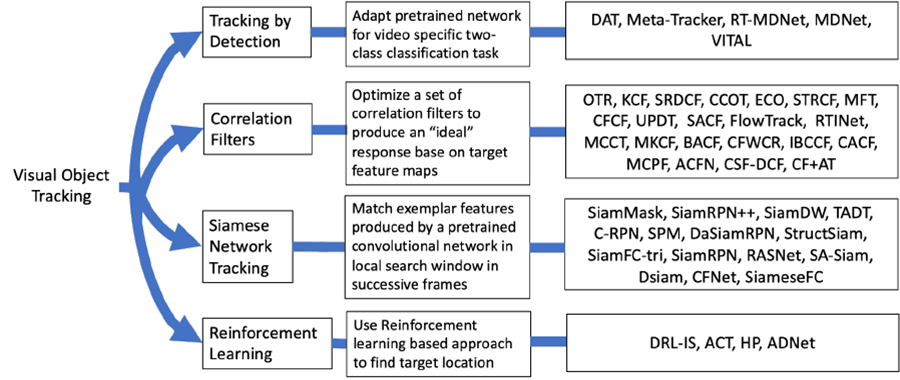
\includegraphics[width = .9\linewidth]{/ip_tracking.png}
 	\caption{Object Tracking Algorithms\cite{s20020547}}
        \label{fig:moment}
 \end{figure}
\FloatBarrier
\justify TD-based algorithms treat tracking as a classification problem and, generally, online training is done so these algorithms run slower. In CF-based algorithms, mostly,  handcrafted or CNN-based features are extracted from the bounding box of the detected object. Then, these features are utilized to obtain a response map at the target location. Although CF-based algorithms  are advantageous in terms of their computational efficiency, even on CPU, they may fail in challenging scenarios that exist in the competition such as fast motion, small object, viewpoint change. SN-based trackers learn the representation of two input images in a similarity fashion, and tracking is achieved with similarity function. An earlier example of this approach is SiamFC. It localizes the exemplar image within the larger image with a fully-convolutional architecture\cite{bertinetto2016fully}. These algorithms require GPU but they run with the higher speed with relatively higher precision because of their offline learning method and we do not need to create a dataset with high frame per second for training the model. Indeed, we can use pretrained weight for the tracking algorithm since the tracking algorithms are class agnostic solutions. Lastly, the RL-based tracker does not achieve desired accuracy \cite{isaac2021unmanned}. 
\justify It is concluded to use a SN-based object tracking algorithm since recent SN-based networks offer higher precision with high speed, and they can even operate real time \cite{shen2022real} on an embedded system. Specifically, DaSiamRPN network will be used due to its distractor aware training and accurate localization with region proposal network as in RCNNs.Also, we are able to use pretrained weights ,which are trained with 250.000 annotated frame, which is far beyond what we can build in this constraint. Moreover, DaSiamRPN outperform deep learning based tracker in 3 out of 4 aerial datasets \cite{isaac2021unmanned} without compromising the speed. 

\paragraph{Dataset}
\justify In order to train the detection algorithm a dataset containing flying RC drones is created. The videos are obtained on YouTube, and two frames are saved for every second. This method provides approximately 10,000 unique frames which are later labeled one by one in Yolo format using labelImg program.
\justify During the selection process of the videos, the variety in terms of the size of the UAV, background, weather condition and resolution is taken into consideration so that the detection algorithm would work in different cases and not overfit.

\justify Also, to increase the size of the dataset, and to decrease the possibility of overfitting to some extent, data augmentation is applied. With the help of this technique 10,000 artificially created frames are obtained, and in total there would be 20,000 frames. The dataset is separated into three parts: train, test and cross validation. 96\% of the dataset is allocated for training, 2\% of it is dedicated for cross validation, and the remaining 2\% is set aside to evaluate the performance of the detection algorithm. The distribution of the data into those three parts is done purely randomly so that there would not be any bias towards any particular configuration throughout the training the network or evaluating the performance of the network.
\justify Some augmentation transformations we used are rotation, saturation change, contrast change, affine, random blur and flip. To augment the existing data, a python library called as albumentations is used. The main advantage of this library is different from many other software and websites, it automatically modifies the annotation files according to the transformation applied on the corresponding frames. 

\begin{figure}
\centering
\begin{subfigure}{.6\linewidth}
  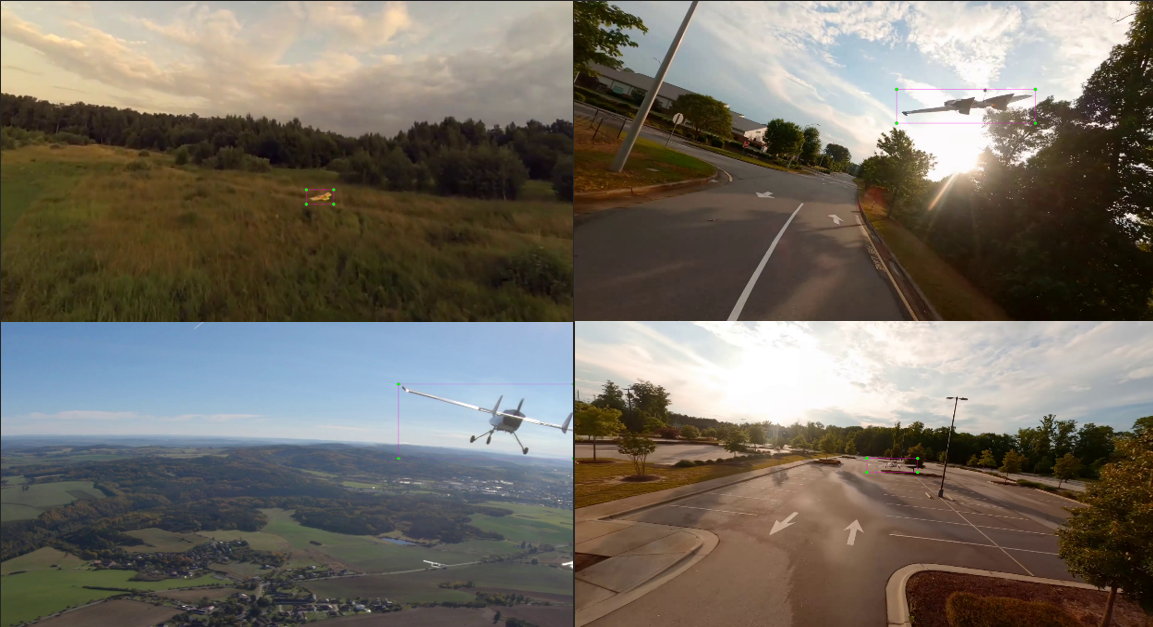
\includegraphics[width=.75\linewidth]{dataset1.png}
  \caption{}
  \label{fig:sub1}
\end{subfigure}%
\begin{subfigure}{.6\linewidth}
  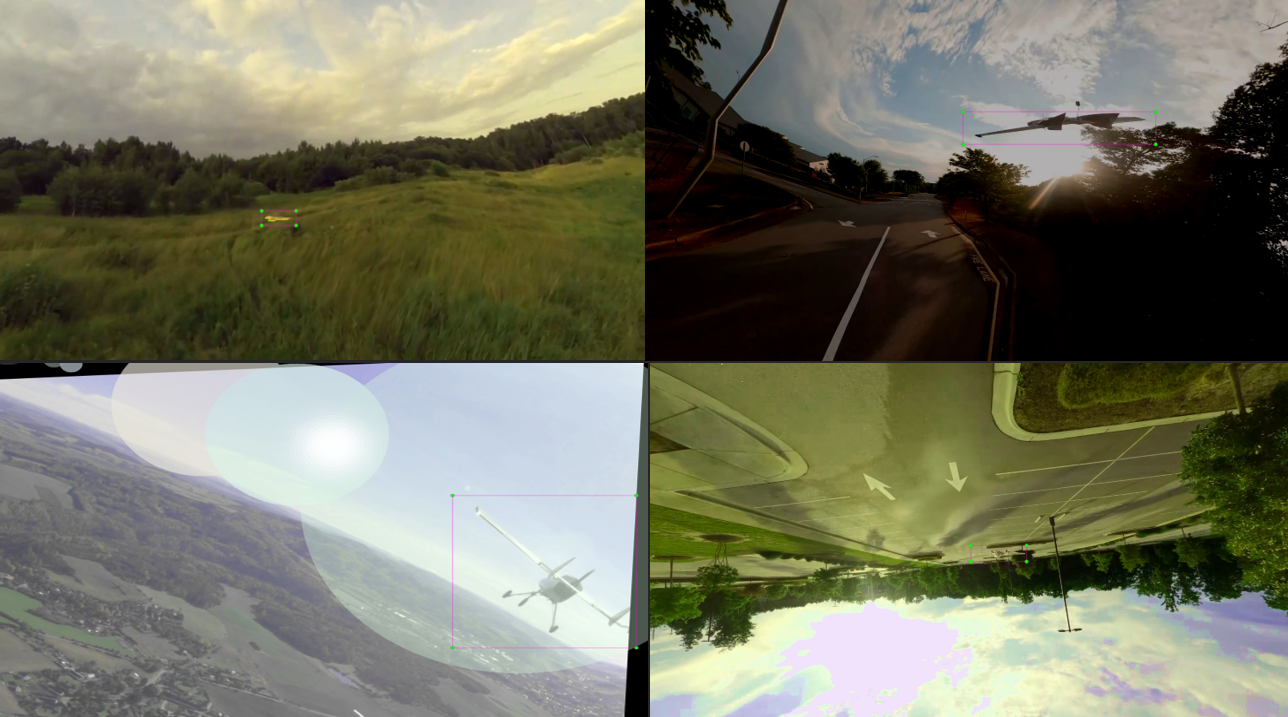
\includegraphics[width=.75\linewidth]{dataset2.png}
  \caption{}
  \label{fig:sub2}
\end{subfigure}
\caption{Examples of dataset samples}
\label{fig:test}
\end{figure}
\FloatBarrier

\subsubsection{Vision-based Guidance}
\justify Firstly, let us discuss the difference between control, guidance and navigation since these terms are often (incorrectly) used interchangeably. Control refers to the applied change in forces to maintain stability of the vehicle and to execute the guidance commands. Similarly, navigation refers to determination of the vehicle’s location, velocity, and attitude. In contrast, guidance includes determination of the optimal path of travel from the vehicle’s current location to a designated target while ensuring a specific velocity, acceleration, and rotation.
\justify Hence, guidance can be considered as the driver of a vehicle. It acts as the intermediary between the navigation system and the control system. The inputs to the guidance system are the outputs of the navigation system (where am I?) and target information (what is my destination?) whereas the outputs are the signals to the flight control system to steer the vehicle accordingly. In the case of our fighting UAV, the inputs will be position, velocity, and attitude of the target UAV obtained using the onboard sensors and object tracking methods discussed earlier. 
\justify Among the numerous benefits of using a PX4 controller, an extremely useful one is the PX4 flight stack. The flight stack includes controllers for fixed wing, multirotor and VTOL configurations along with estimators for the position and attitude. The diagram below neatly summarizes the constituents of the flight stack.

\begin{figure}[ht]
 	\centering
 	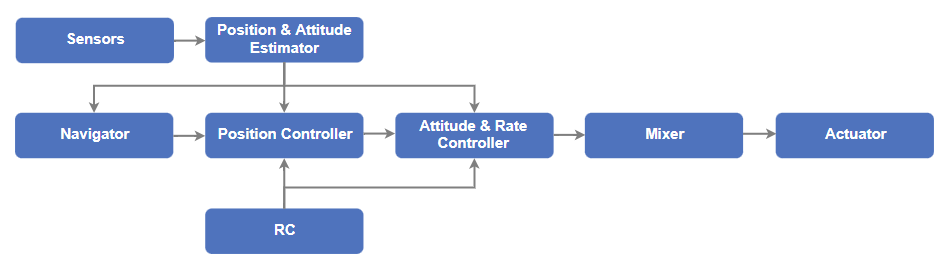
\includegraphics[width = .9\linewidth]{/control1.png}
 	\caption{The building blocks of the PX4 flight stack. \cite{px4}}
        \label{fig:blocks_PX4}
 \end{figure}
 %references should be rearranged ! 
\FloatBarrier
\justify Let us have a deeper look at some of the vital components in Figure \ref{fig:blocks_PX4} above. 
\justify The estimator takes one or more sensor inputs, combines them and returns a vehicle state. In the case of a fixed-wing UAV, the attitude and position estimators use an Extended Kalman Filter (ekf2). The EKF is a nonlinear version of the Kalman Filter (KF) which is a powerful tool in guidance, control, and navigation of vehicles. The Kalman Filter stores the estimated state of the system along with the uncertainty of the estimate. This estimate is updated using a state transition model and measurements coming from sensors in our case. Hence, unknown variables are estimated more accurately compared to single measurements. 
\justify The controllers take setpoints and the estimated states as input. The goal of the controller is to adjust the input in an optimal way such that the output corresponds to the setpoint. We will be discussing the various controller algorithms in the coming subsection. 
\justify Finally, the mixer block above divides each task into meaningful inputs for individual motor components and ensures that the actuators are not saturated. 
\justify As mentioned earlier, the position, velocity, and attitude of the target UAV will be determined with the help of the camera. The position and velocity will be fed as setpoints to the Fixed Wing Position Controller module. The Total Energy Control System (TECS) within this module enables simultaneous control of the true airspeed (TAS) and altitude of a fixed-wing aircraft. 
\begin{figure}[ht]
 	\centering
 	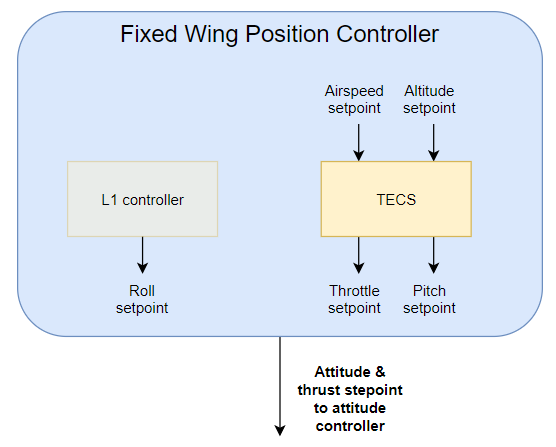
\includegraphics[width = .7\linewidth]{/control3.png}
 	\caption{The fixed wing position control module. \cite{px4}}
        \label{fig:moment}
 \end{figure}
\FloatBarrier
\justify As shown in the Figure above, the TECS takes the airspeed and altitude as input and outputs the throttle and pitch angle setpoints. These setpoints are then input for the fixed wing attitude controller (explained later) to implement the attitude solution. Similarly, the L1 controller for fixed wing is for the lateral control of the UAV and returns the roll setpoint to be used by the fixed wing attitude controller.
\justify It is important to note that the simultaneous control of the height and the true airspeed is a challenging control problem. This is because an increase in the aircraft pitch angle will cause an increase in the height but a decrease in the true airspeed. Similarly, increasing the throttle setting results in a higher true airspeed but the height also increases. Thus, the two inputs to the position controller (pitch angle and throttle setting) influence the two outputs (true airspeed and altitude). 
\justify To decouple the control problem, the TECS algorithm represents the problem in terms of energies rather than the original setpoints. The total energy of the system is simply divided into kinetic and potential energy. This way, each maneuver and configuration can be achieved using an appropriate combination of kinetic and potential energies. An example of this is how flying at a slow speed but higher altitude is equivalent to flying at a faster speed but a lower altitude. This is referred to as the specific energy balance and it is solely governed by the pitch angle. Similarly, the throttle setting regulates the specific total energy of the vehicle. This way, the positon control problem is decoupled and controlled independently. 
\justify Moreover, PX4 also offers a Fixed-Wing Attitude Controller. The attitude controller follows a cascaded loop architecture. The outer loop determines the error in attitude between estimate and setpoint, multiplies this with the gain (proportional controller), and returns a rate setpoint. Similarly, the inner loop computes the error in the corresponding rates and makes use of a PI controller (proportional and integral) to return the deseried angular acceleration. This controller is illustrated in Figure \ref{fig:attitudecontrol} below.
\begin{figure}[ht]
 	\centering
 	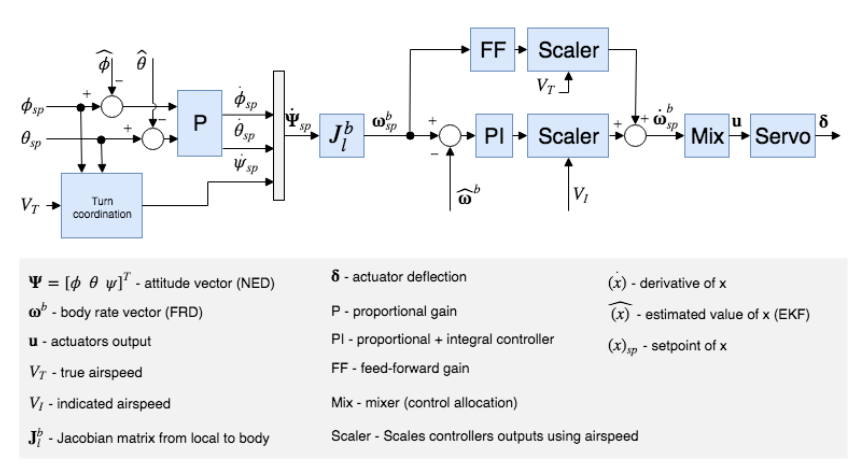
\includegraphics[width = .9\linewidth]{/control2.png}
 	\caption{The fixed-wing attitude control module}
        \label{fig:attitudecontrol}
 \end{figure}
\FloatBarrier
\justify The angular acceleration setpoint is then used to calculate the angular position of the actuator surfaces with the help of the mixer (discussed earlier). Other aspects of the controller include a scaler to scale the airspeed measurements (if such a sensor is available onboard) and the feedforward gain to compensate for aerodynamic damping. An additional note here is that the yaw controller generates its setpoint using the turn coordination constraint while the longitudinal and lateral dynamics is assumed to be uncoupled. 
\justify Once the vehicle gets close enough to the target UAV (greater than 5 percent of the frame), we will directly use the attitude of the rival UAV and ensure that the target area is within the target shooting area as described in the competition guidelines. This part will require the use of MATLAB/Simulink combined with the ROS2 toolbox. The simulation environment for testing will be Gazebo.

\subsection{Kamikaze Mission}
\justify In this mission, the vehicle is expected to perform nose dives on ground targets whose coordinates are given and retrieved by scanning a QR code. In this case, only the positions of the ground targets will be sufficient since they are stationary. Again, the position, altitude and velocity can be given to the TECS algorithm as setpoints. Once the vehicle locks on to a ground target, it will approach it in a diving maneuver until the scan is complete. These conditions can easily be applied in the MATLAB/Simulink environment and communicated with PX4 using ROS2. Also, for the scanning, OpenCV and pyzbar libraries will be utilized.
\justify To fulfill the kamikaze mission, the Astrotech UAV climbs approximately to 75 meters so that when it starts to dive, it would be possible to maintain visual contact with the target for a sufficient period of time to scan. Additionally, in order to minimize the velocity of the UAV during the dive, the motors would not be activated, and it would fall freely. It is also given that the QR code is surrounded by plates having an angle of 45 degrees, and taking into consideration the angle of view of the camera, which is approximately 20 degrees, the dive should be performed by 25 degrees with the ground. When the QR code is scanned successfully it would start to perform a vertical circular motion in order to recover from the diving and start to elevate.
\justify In order to minimize the risk of collision, the Astrotech UAV would perform less aggressive maneuvers. To further explain, if the Astrotech UAV scans the QR code before reaching a threshold altitude, it immediately starts the vertical circular motion. However, if it reaches the threshold altitude, which is 20 meters above the ground, without scanning the QR code, the mission will be aborted, and  it will start a recovery maneuver. If that would be the case, the altitude to start the diving would be increased by approximately 20 meters in each unsuccessful attempt.
\justify Considering the scanning process cannot be done in the first attempt, diving altitude gets higher and higher. In the worst case scenario, it is predicted that as a result of the free falling, the velocity of the Astrotech UAV would approximately be 45 m/s when the recovery maneuver starts. Considering the velocity and the radius of turn, the Astrotech UAV would undergo a maximum of 3 g upward acceleration. The calculation is done by the using the following formula:
%Buraya formüller gelecek

\begin{align}
    L - W = (\frac{mv^2}{R}) & \ \ \xrightarrow{}& &n = (\frac{v^2}{gR}) +1 \\
    R = 10+ R \times \cos(25^{\circ}) &\ \ \xrightarrow[]{}& & R \approx 107 \ meters\
\end{align}
\justify The structural test shows us that the frame can withstand up to 3.5 g, which means performing the recovery maneuver with these configurations, such as diving altitude, turn radius, etc., would not pose any threat for the Astrotech UAV.

\section{GROUND STATION AND COMMUNICATION}
Under this topic, the details about in-vehicle communication, vehicle-ground station communication and ground station to main server communication are given.
\subsection{In-Vehicle Communication}

\begin{figure}[ht]
 	\centering
 	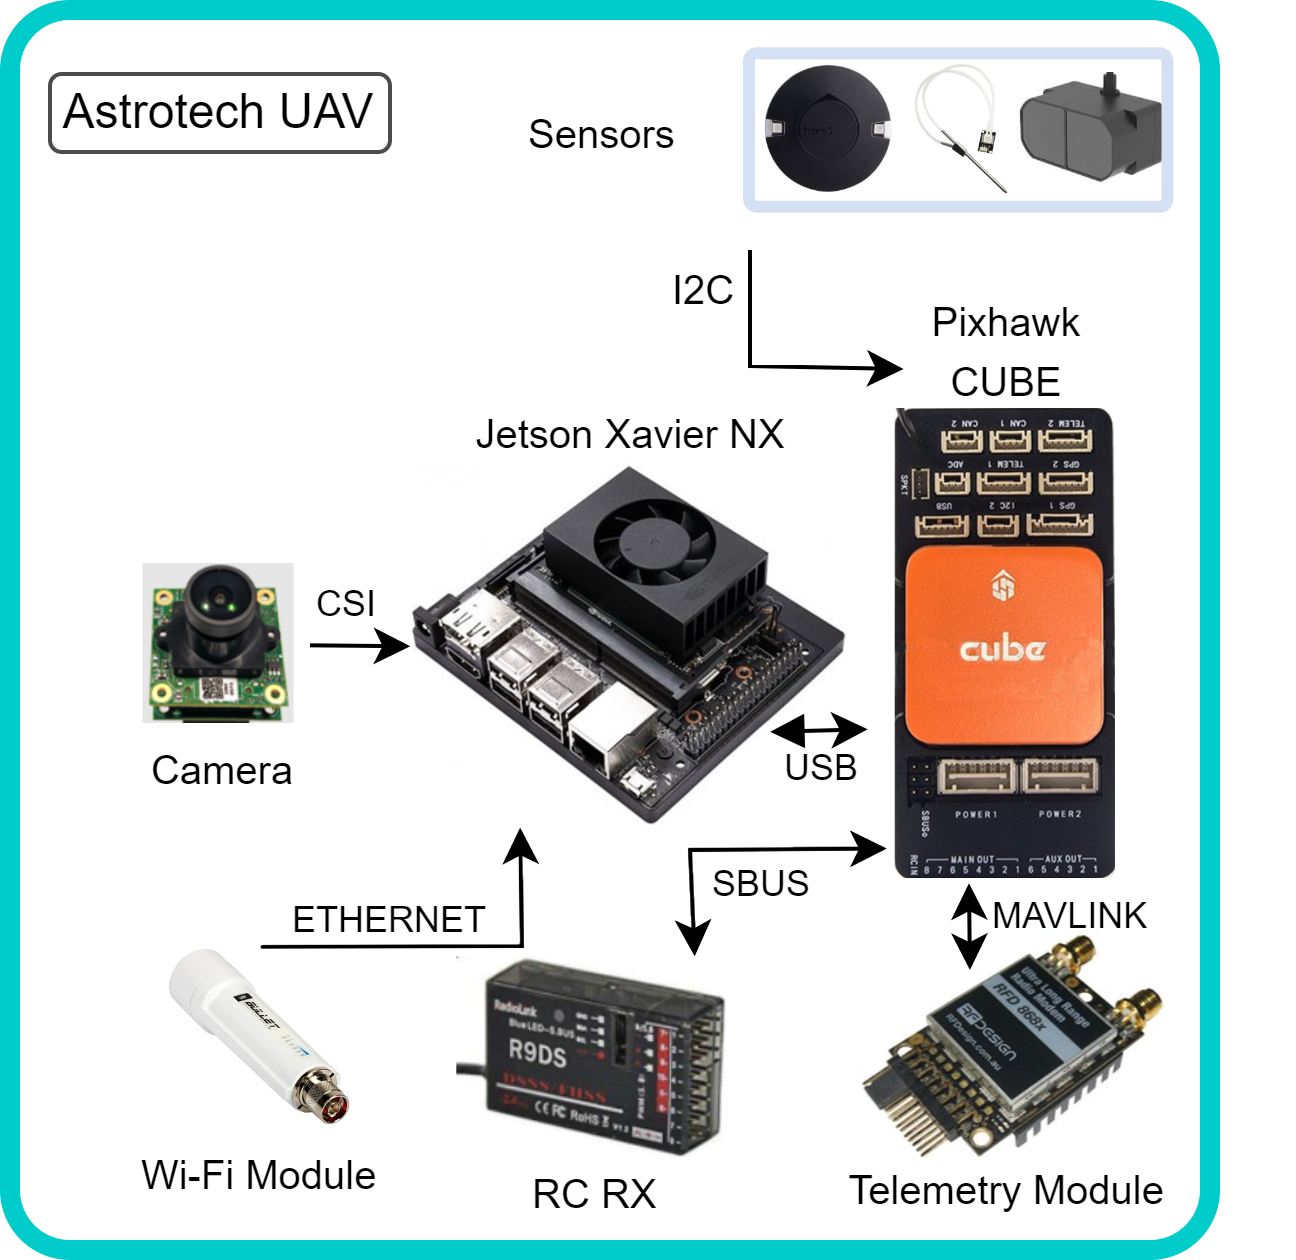
\includegraphics[width = .5\linewidth]{unnamed (24).png}
 	\caption{Astrotech UAV in-Vehicle Communication Diagram}
        \label{fig:in_veh_com}
 \end{figure}
\FloatBarrier

\paragraph*{Camera-Companion Computer Communication:} Communication between e-CAM24\_CUNX and Nvidia Xavier NX is based on CSI-2 MIPI communication specification. FPC connector is used to establish the connection. This connector allows the camera output port to be connected to the Camera0 (or Camera1) port of Xavier NX.

\paragraph*{Companion Computer-Flight Control Card:} The communication of Xavier NX and Pixhawk Cuber Orange takes place according to UART, which is an asynchronous serial communication protocol. The sent data packages are prepared according to the MAVLink data protocol, and Fast RTPS (Real Time Publish and Subscribe) is also used for fast access. For this to be possible, it requires the use of the PX4-Fast RTPS(DDS) Bridge. In order to establish the hardware connection, it is necessary to connect the one side of connector to the Telemetry0 or Telemetry1 port of Pixhawk Cube Orange and then the relevant lines of it to the RX, TX, 5V and, GND ports of Xavier NX.

\paragraph*{Flight Controller-GPS:} Communication between Pixhawk Cube Orange and Here3 GPS takes place according to CAN protocol. Here3 GPS connector is connected to CAN port of Pixhawk Cube Orange.

\paragraph*{Flight Controller-Airspeed Sensor:} The communication between these components takes place via I2C protocol. To establish the connection, the connector of the Holybro digital airspeed sensor is connected to the I2C port of the Pixhawk Cube Orange.

\paragraph*{Flight Controller-Control Receiver:}Communication between R12DSM and Pixhawk Cube Orange takes place according to SBUS protocol. SBUS is a serial communication protocol used especially in hobby vehicles. In order to establish the connection, the connector of the R12DSM must be connected to the SBUS port located at the beginning of the servo line of the Pixhawk Cube Orange.

\paragraph*{Flight Controller-Telemetry Module:} Communication between Pixhawk Cube Orange and RFD868 will take place according to UART communication protocol. The data packages sent have a form suitable for the MAVLink communication protocol. In order to establish the hardware connection, the connector of the RFD868 is plugged into the Telemetry0 or Telemetry1 port of the Pixhawk Cube Orange. 

\paragraph*{Flight Controller-ESC-Servo Motors:} Control outputs from Pixhawk Cube Orange are transmitted to ESC and servo motors as PWM signals.

\subsection{UAV-Ground Control Station Communcation}
\begin{figure}[ht]
 	\centering
 	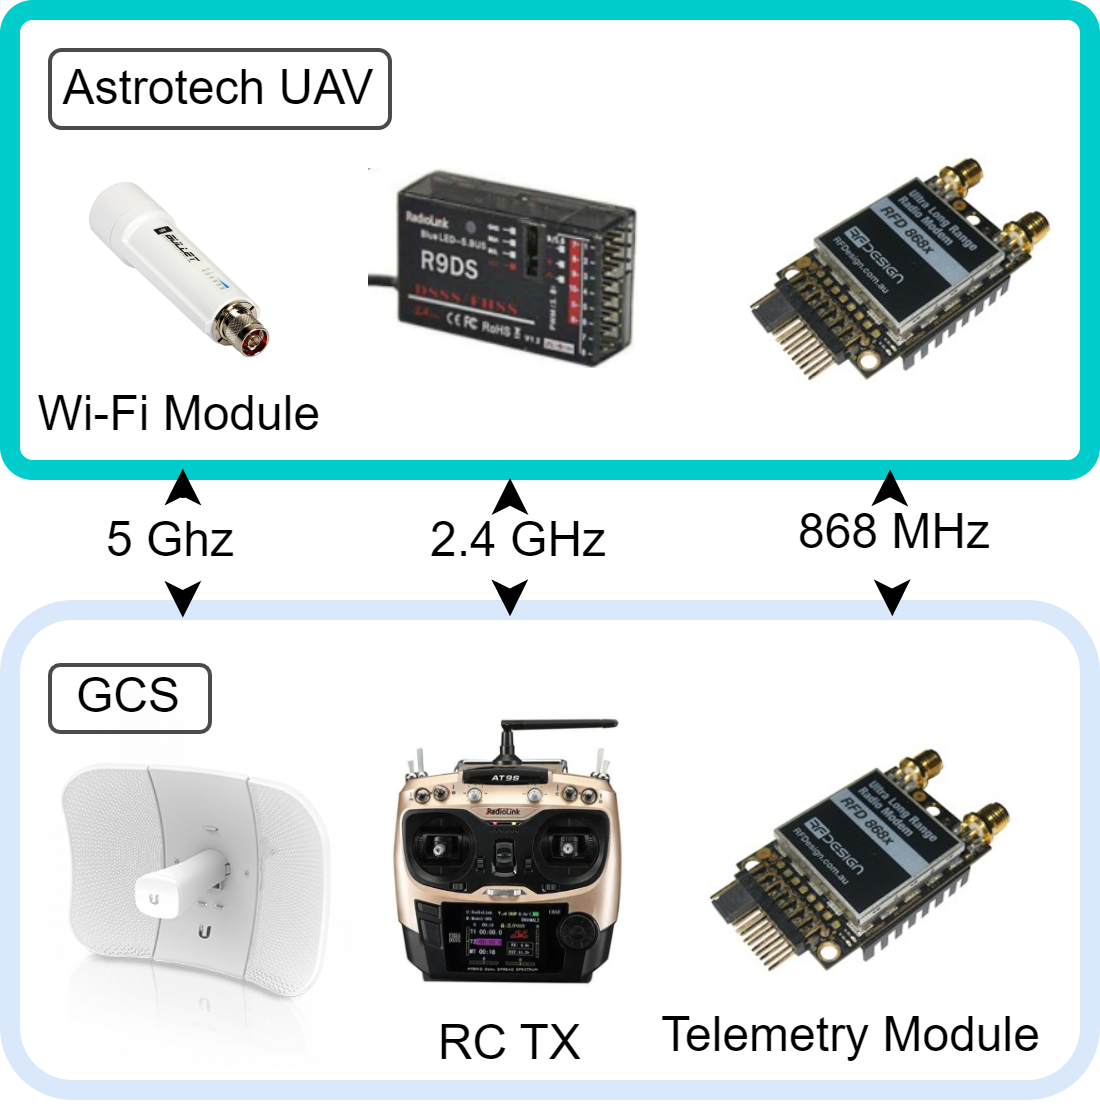
\includegraphics[width = .5\linewidth]{/unnamed (25).png}
 	\caption{Astrotech UAV-Ground Station Communication Diagram}
        \label{fig:assembly_side}
 \end{figure}
\FloatBarrier
\paragraph*{RFD868 Modules:} The frequency range of these modules is 865-870 MHz and they enable RC PPM Passthrough with telemetry at the same time. When connected to Pixhawk, data packages are transmitted to the ground station according to the MAVLink communication protocol. They have a default Air Data transfer rate of 64 kbit/s and support up to 750 kbit/s. The connection between the RFD868 module used in the ground station and the ground station computer will be made via the USB port. Incoming data is packaged according to the MAVLink data protocol. These data coming to the ground station are used to update the interface with the pymavlink library.

\paragraph*{Ubiquiti Bullet M5-HP 5Ghz - LiteBeam-5AC-GEN2 Communication:} Communication between these two modules takes place at 5.8 GHz. Omni-directional data transmission is provided by using mushroom antenna on Bullet M5. The LiteBeam-5AC-GEN2 used in the ground station has an antenna having greater gain. The connection between the module and the ground station computer will be provided with an Ethernet cable. Thanks to this LAN connection, the video coming from the camera can be followed from the ground station.

\paragraph*{AT9S PRO-R12DSM:} The connection between the controller and the receiver takes place on the 2.4 GHz band. R12DSM has 12 channels and this is enough for the requirements of the design. 

\paragraph*{RTK Module Connection:} Here+ RTK module is connected to the ground station computer via USB port.

\subsection{Ground Control Station Main Server Communication}
Communication in HTTP protocol will be provided in order to be able to access data about rival UAVs coming to the main server and to transfer the requested information of Astrotech UAV to the main server. The standards of communication will be determined by the competition committee. Hardware connection will be established via ethernet cable.

\section{USER INTERFACE DESIGN}
In this section, design of the interface/s that will be used on ground control station should be explained. İnformations about the flight such as speed, altitude, mode change, and locking rectangle must be shown on the interface.

\justify
Astrotech Ground Station consists of two separate units in order to provide the necessary controls for the flight and to transmit the command for the missions:

\begin{itemize}
	\item Open Source Ground Control Software
	\item Astrotech UAV
\end{itemize}

It is suitable to run in Ubuntu operating system due to the ease of use of UNIX with ground control station software architecture and the used computer has Ubuntu operating system.

\subsection{Ground Control Software (QGroundControl)}
QGround was preferred because the Astrotech platform is accustomed to be used during the tests and our team has experience with it. QGround provides full flight control and configuration for ArduPilot or PX4 Pro powered vehicles. It also provides mission planning for autonomous flight. QGroundControl, which has an easy and understandable interface, has been found suitable for use.     \\ 
\begin{figure}[ht]
 	\centering
 	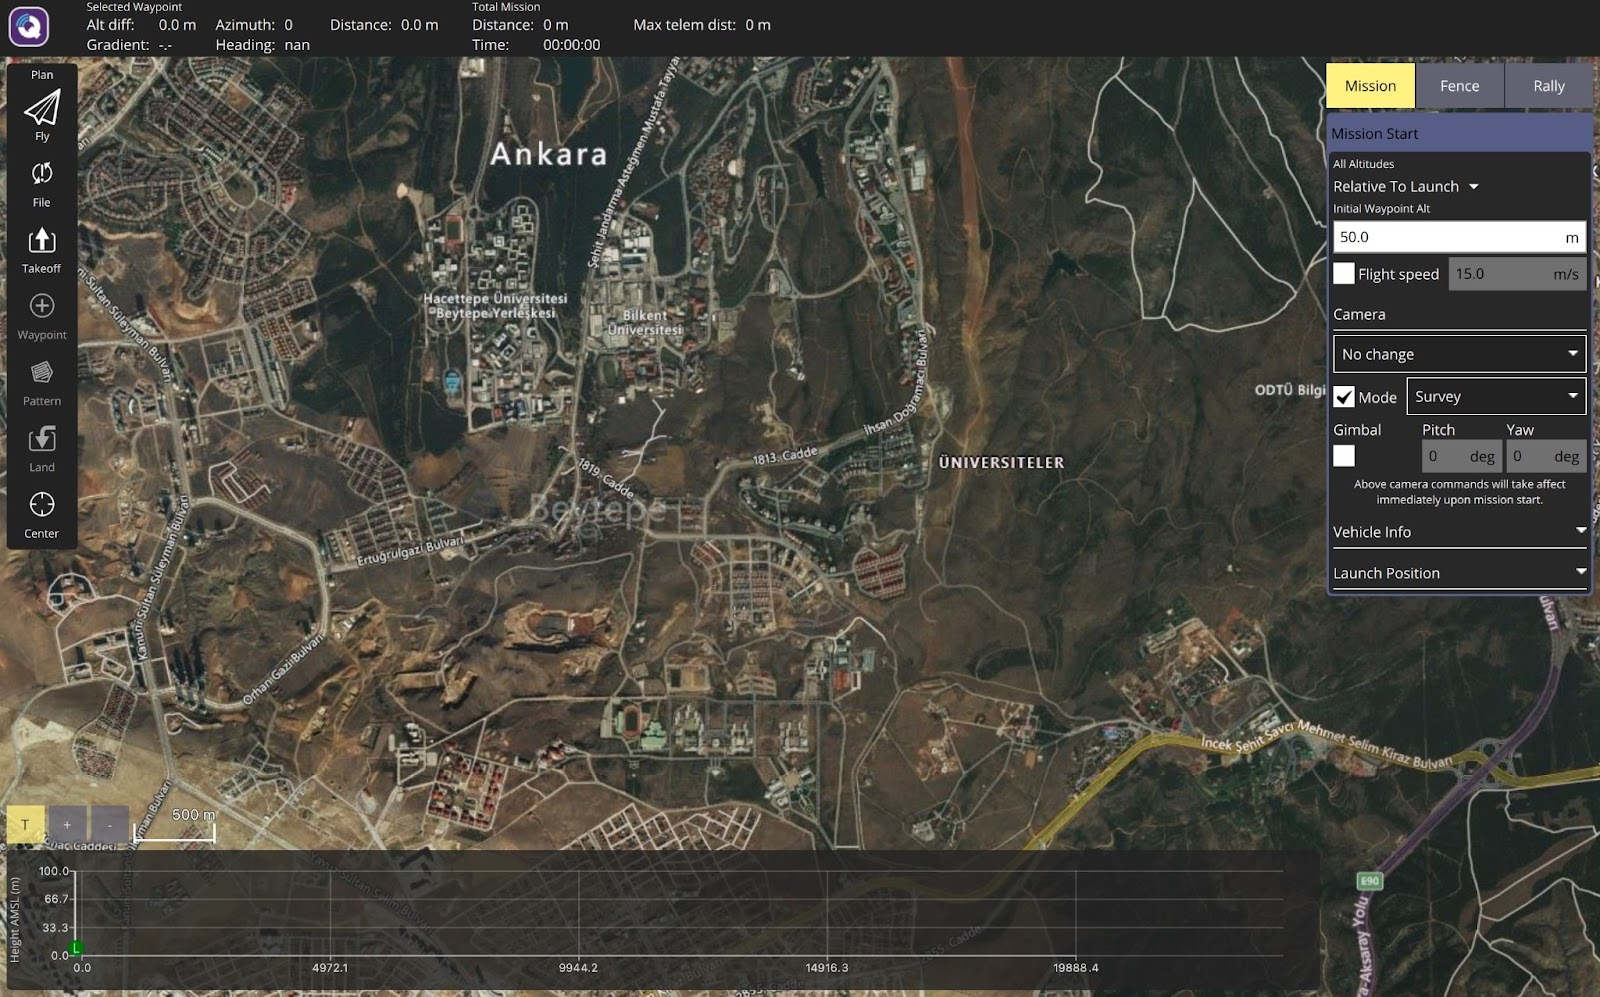
\includegraphics[width = .8\linewidth]{/gcs1.jpg}
 	\caption{QGroundControl User Interface}
        \label{fig:Q_ground}
 \end{figure}
\FloatBarrier
\justify 
In addition to displaying the dynamic, electronic, and location features of the UAV in real-time, it also has a flight planner for autonomous missions. During the competition, features such as direction, position, height, distance, and battery voltage obtained on the Astrotech’s platform will be controlled over the QGroundControl interface, and emergency response commands will be transmitted over QGround for possible needs.

\subsection*{Astrotech User Interface}
The commands to provide the desired conditions during the competition are integrated into the Astrotech interface. Mode change, opponent selection, landing, and take-off situations with the provided commands can be determined by Astrotech interface. It supports the ground station in terms of easy usage and usability.     
\justify
     Images from the CSI Deadlock Camera will be able to be followed from astrotech user interface. After locking square is created, the image will be transferred to the ground control software by opencv library.
\justify

       The location informations from the server will be displayed on a virtual coordinate planes between Astrotech and competitor UAVs. autonomous locking, the route to be followed by Astrotech in the air will be followed in real time through the radar system we use these coordinates. The traceable route is shown as in the Figure \ref{fig:Minimapwidget}. The x-axis shows longitude, while the y-axis shows latitude.
      For autonomous locking, locking to the competitor can be selected autonomously, while it can also be selected manually from the ground control center.
      With the help of the control screen, the desired requests can be fulfilled easily. It has the feature to be controlled from the ground station with QgroundControl in case of emergency.
      \clearpage


\begin{figure}[]
     \centering
     

     \begin{minipage}[b]{0.39\textwidth}
         \centering
         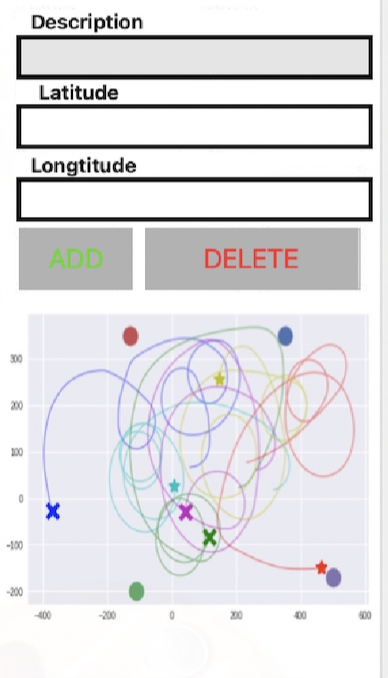
\includegraphics[width=\textwidth]{gcs2.png}
 	    \caption{Minimap widget}
 	   \label{fig:Minimapwidget}
       \end{minipage}
     \hfill
     \begin{minipage}[b]{0.6\textwidth}
         \centering
         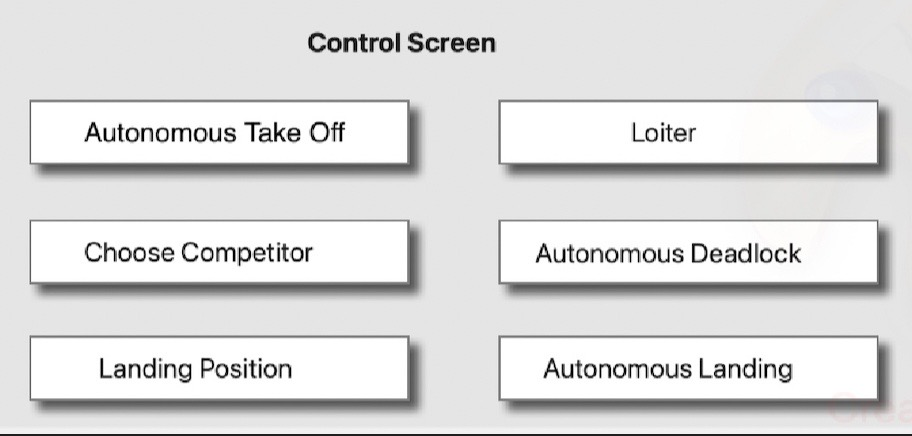
\includegraphics[width=\textwidth]{gcs4.jpg}
        \caption{Command buttons}
         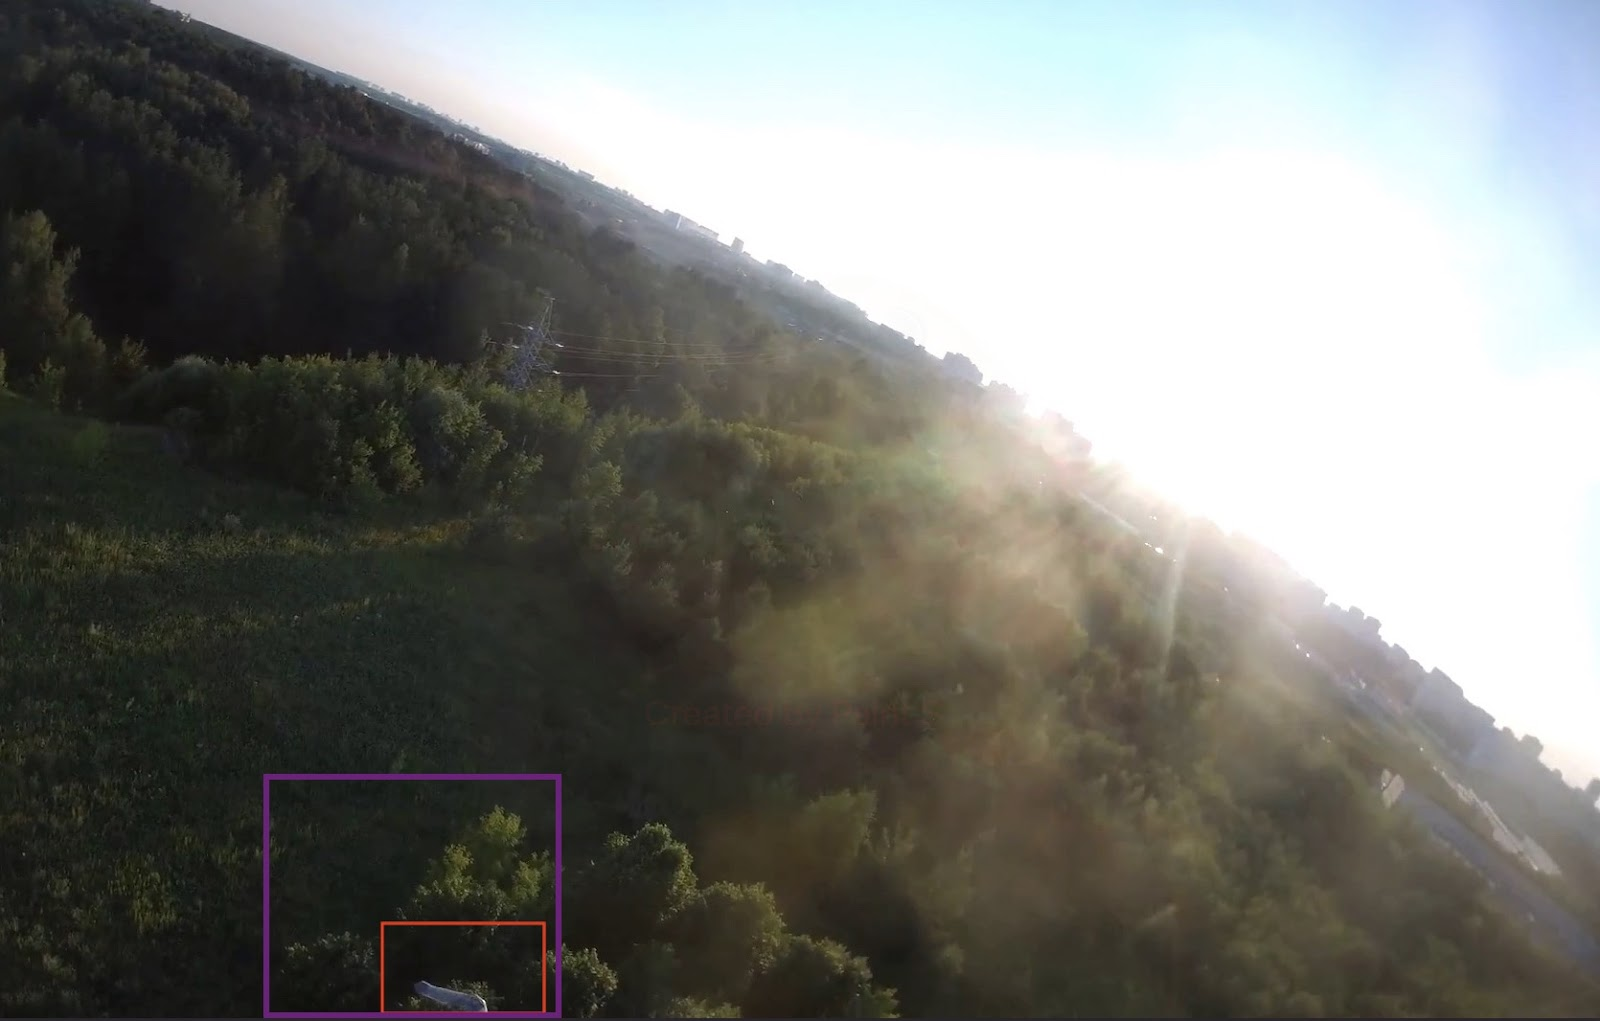
\includegraphics[width = \textwidth]{gcs5.jpg}
        \caption{CSI Deadlock Camera Feed}
     \end{minipage}
     \hfill
     
     \caption{Widgets in Astrotech GCS}
    \label{fig:three graphs}
\end{figure}

\justify
We can also follow some values such as longitude and latitude like obvious in Figure \ref{fig:Minimapwidget}, and also it stated that it is easy to follow route of the Astrotech UAV and competitors’ UAV.
\justify
\justify
Although electronic and dynamic calculations for flight will be done by QGroundControl, basic flight characteristics such as speed, altitude, and mode can also be followed from the Astrotech interface.

\justify
Astrotech interface is showed in Figure \ref{fig:in_veh_com} Advantages of Astrotech User Interface:
It is easy to use interface
It contains basic commands needed will be able to perform the desired tasks for the ccompetition by communicating with the server.
It can be used for many purposes because it is easy to edit and open to developments.
\FloatBarrier

\begin{figure}[ht]
 	\centering
 	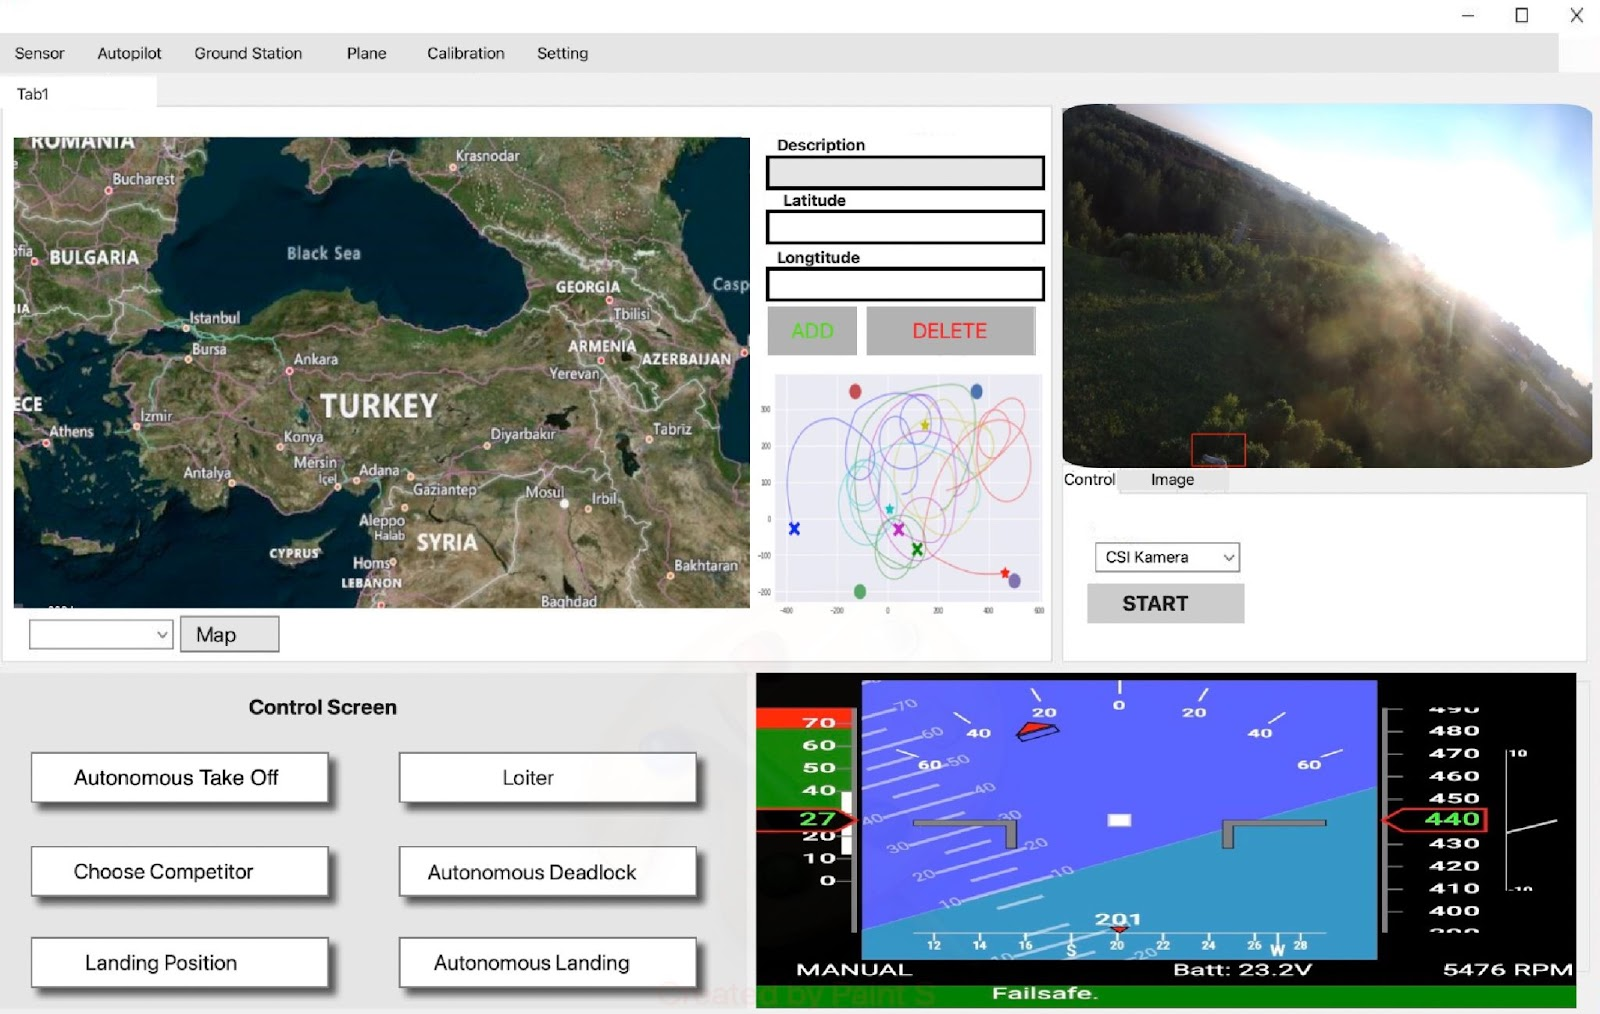
\includegraphics[width = .8\linewidth]{/gcs3.jpg}
 	\caption{Astrotech GCS user interface}
        \label{fig:in_veh_com}
 \end{figure}
\FloatBarrier

\section{AIRCRAFT INTEGRATION}


\subsection{Stuctural Integration}
In this part, the steps to build the X-UAV Talon is explained with images taken in the process. The X-UAV Talon consists of a wooden frame, EPO foam body and wings, and carbon fiber rods for increased structural integrity.

\begin{figure}[ht]
 	\centering
 	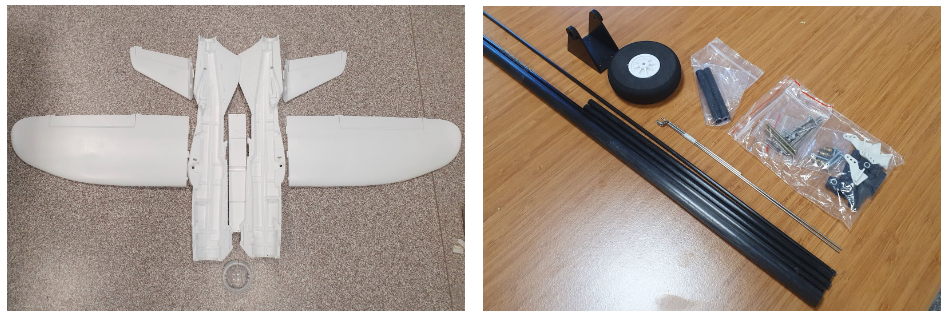
\includegraphics[width=\linewidth]{partsoftalon.png}
 	\caption{Parts of X-UAV Talon}
        \label{fig:in_veh_com}
 \end{figure}
\FloatBarrier

%\begin{figure}
%     \centering
%     \begin{subfigure}[b][3cm]{0.49\textwidth}
%         \centering
%         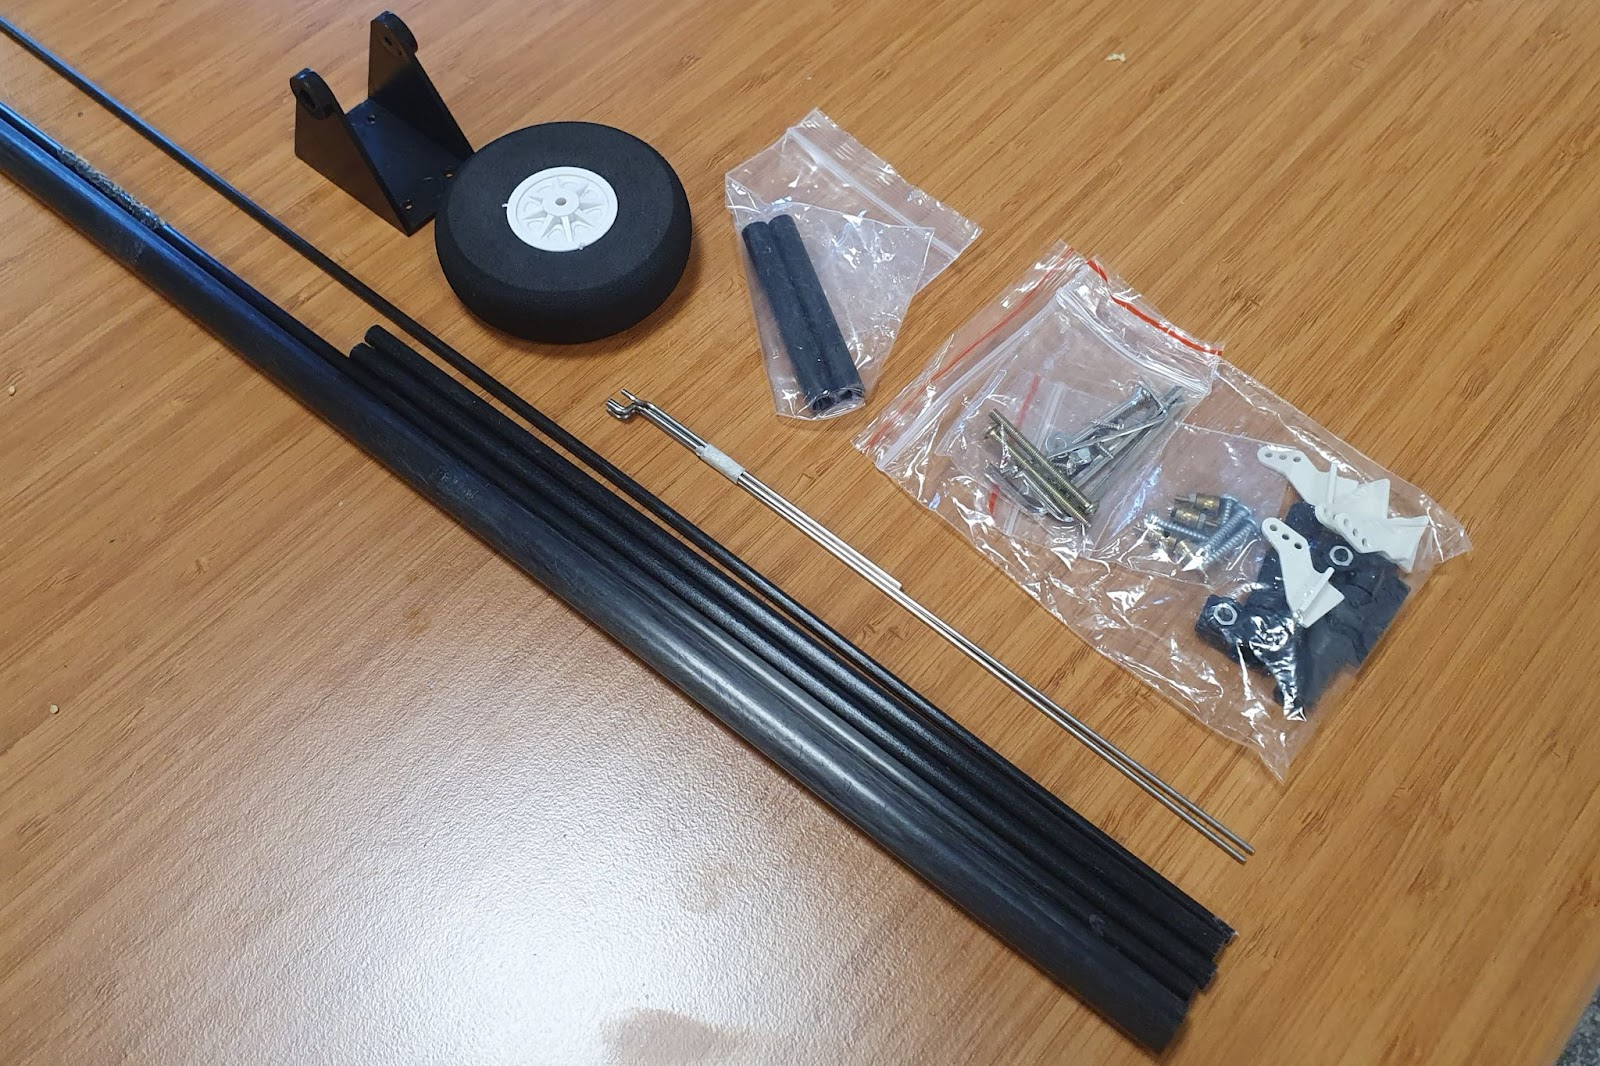
\includegraphics[width=\textwidth]{unnamed (4).jpg}
%%       \end{subfigure}
%     \hfill
%     \begin{subfigure}[b][3cm]{0.49\textwidth}
%         \centering
%         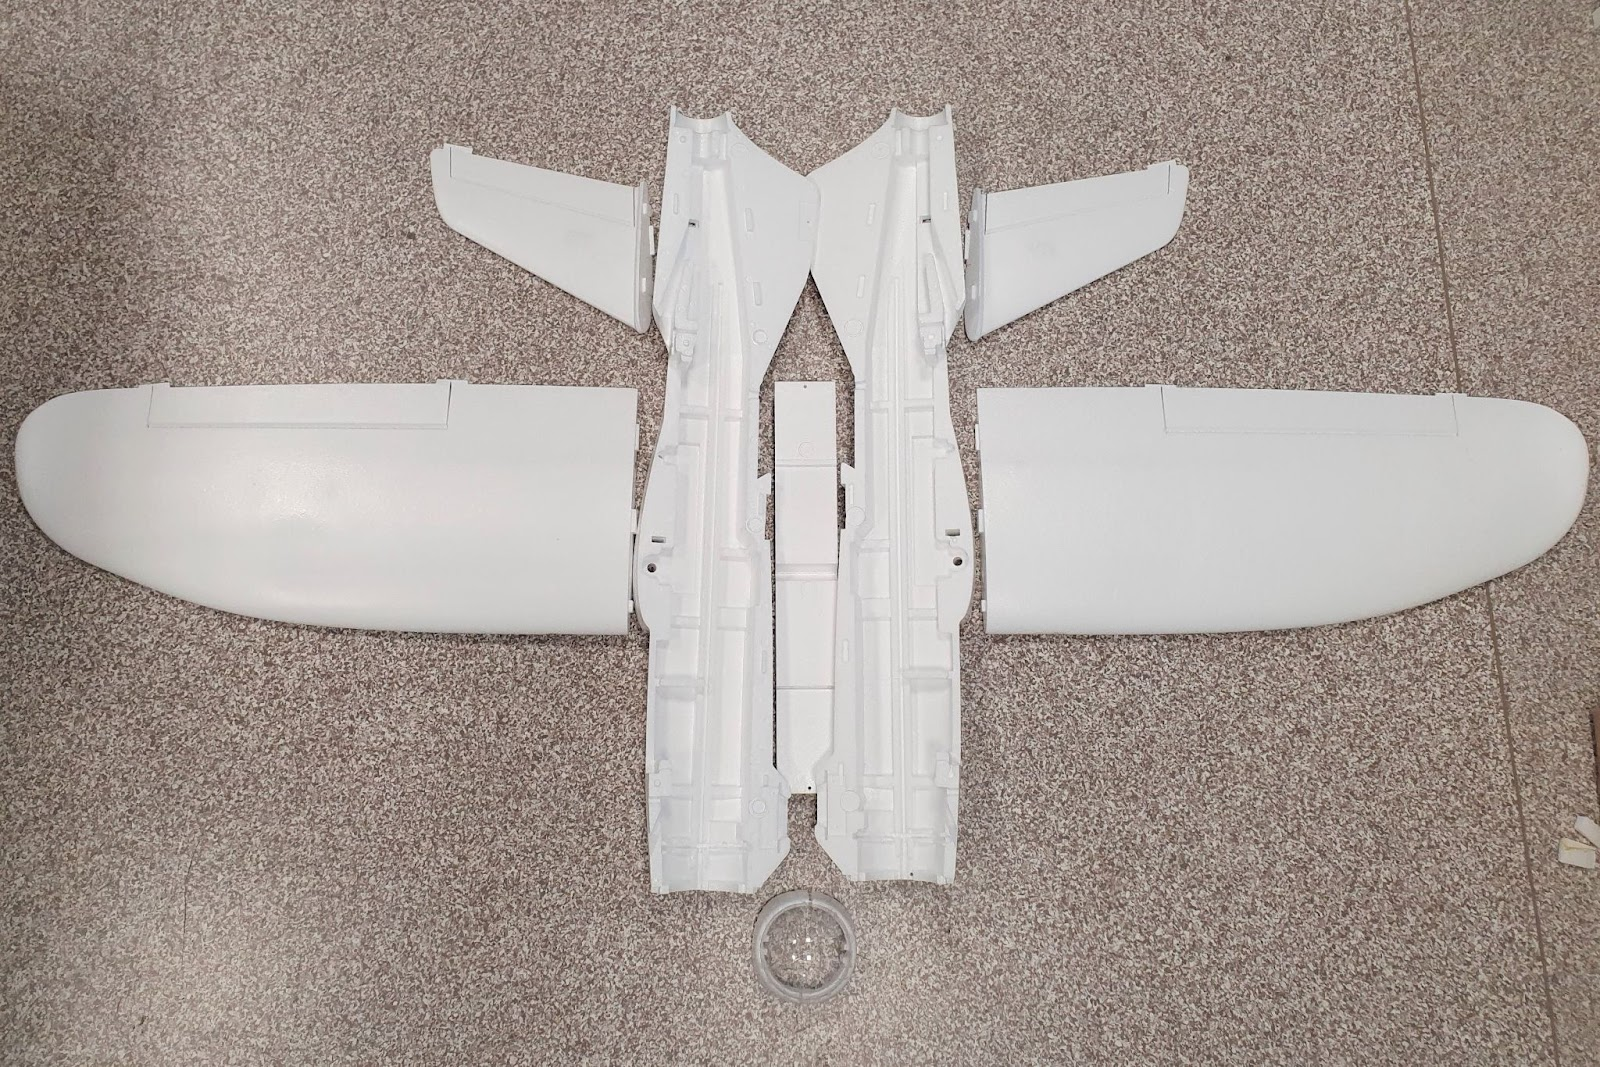
\includegraphics[width=\textwidth]{unnamed (5).jpg}
%     \end{subfigure}
%     \caption{Parts of X-UAV Talon}
%    \label{fig:three graphs}
%\end{figure}
%\FloatBarrier
\justify
As a first step, the plywood pieces that form the inner frame of the aircraft were fixed together with an appropriate wood glue. The parts were secured together and left to dry. This part will hold the foam parts of the fuselage together and it will also be used as a platform to hold the equipment of the aircraft. Then, to prepare the two part fuselage, 6mm carbon fiber rods were glued to their slots. Polyurethane glue is used in steps involving gluing parts to foam. Polyurethane glue bonds parts to foam strongly due to its expanding nature. It is also suitable for our use because it doesn’t react with the EPO foam.
\begin{figure}[ht]
	\centering
	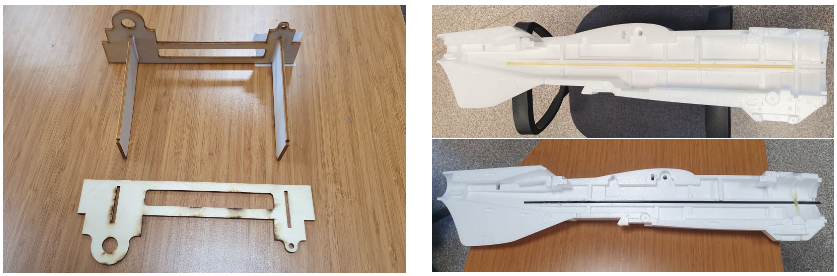
\includegraphics[width = \linewidth]{figures/constuction.png}
	\caption{Construction of the UAV}
       \label{fig:construction}
 \end{figure}
\FloatBarrier


% \vspace{-\abovedisplayskip}
%\FloatBarrier
%\begin{figure}
%\centering
%\begin{minipage}[c][5cm][t]{.49\textwidth}
  %\vspace*{\fill}
%  \centering
%  \includegraphics[width=\textwidth]
%  {figures/unnamed (6).jpg}
%  \caption{The Plywood Frame}
%  \label{fig:test1}
%\end{minipage}%
%\hspace{6pt}
%\begin{minipage}[c][5cm][t]{.49\textwidth}
 % \vspace*{\fill}
 % \centering
 % 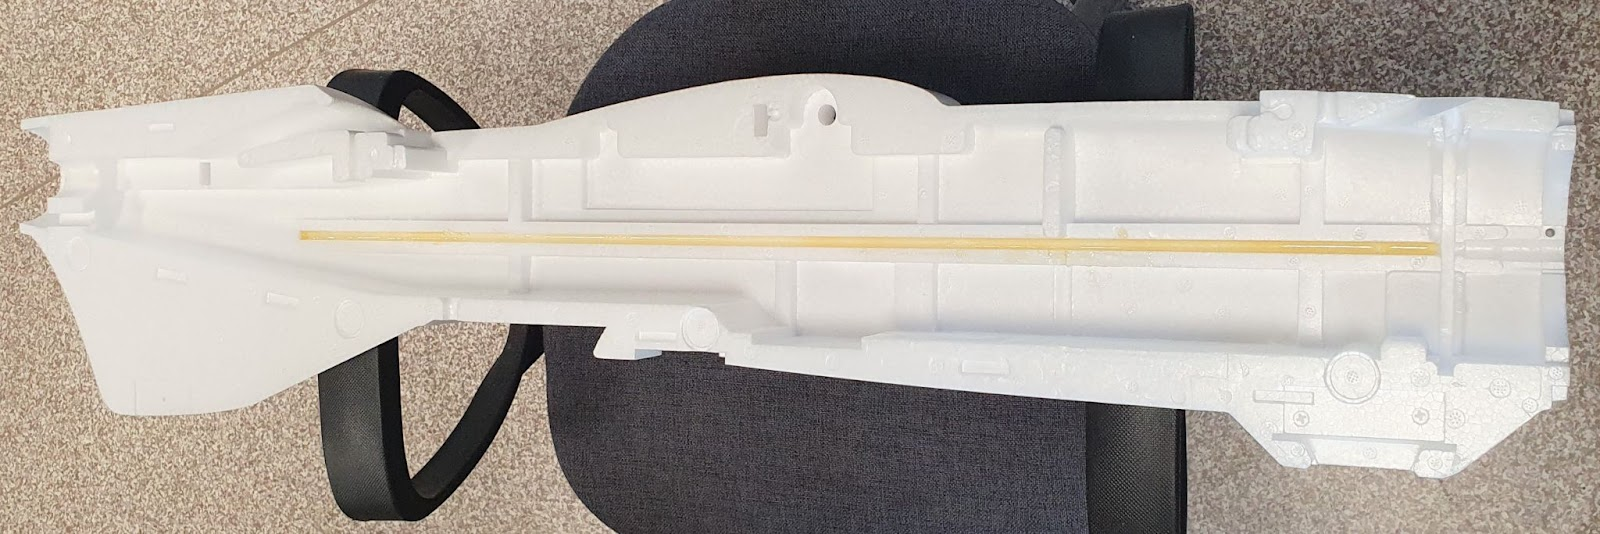
\includegraphics[width=\textwidth]{figures/unnamed (9).jpg}
 % 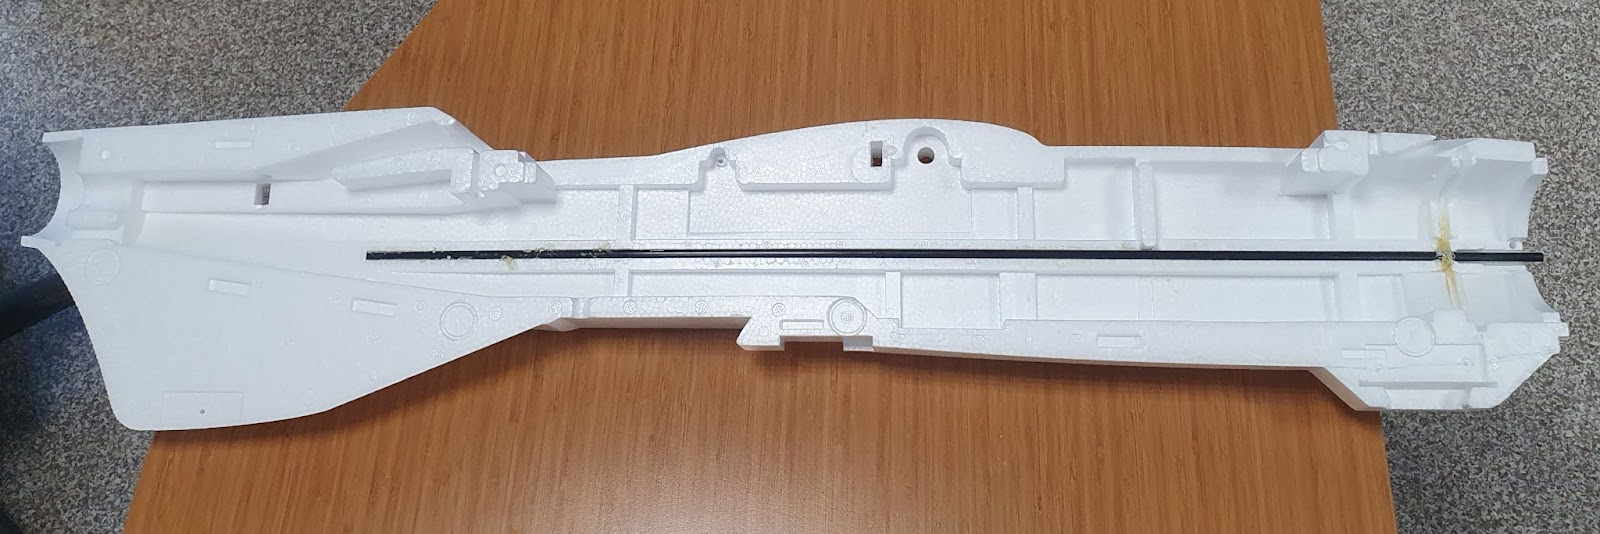
\includegraphics[width=\textwidth]{figures/unnamed (8).jpg}
 % \caption{Gluing Carbon Tube}
%  \label{fig:test3}
%%\end{minipage}
% 
% \end{figure}
\FloatBarrier
\justify
After this step, the frame is ready to be glued to one side of the foam body. After all plywood pieces are fixed, the other side of the body is glued to the rest of the parts to complete the fuselage of the aircraft. In this step, to make sure we have a successful bond, the fuselage was fixed together with paper tape until the glue is completely dry.

%\begin{figure}
%     \centering
%     \begin{subfigure}[b]{0.32\textwidth}
%         \centering
%         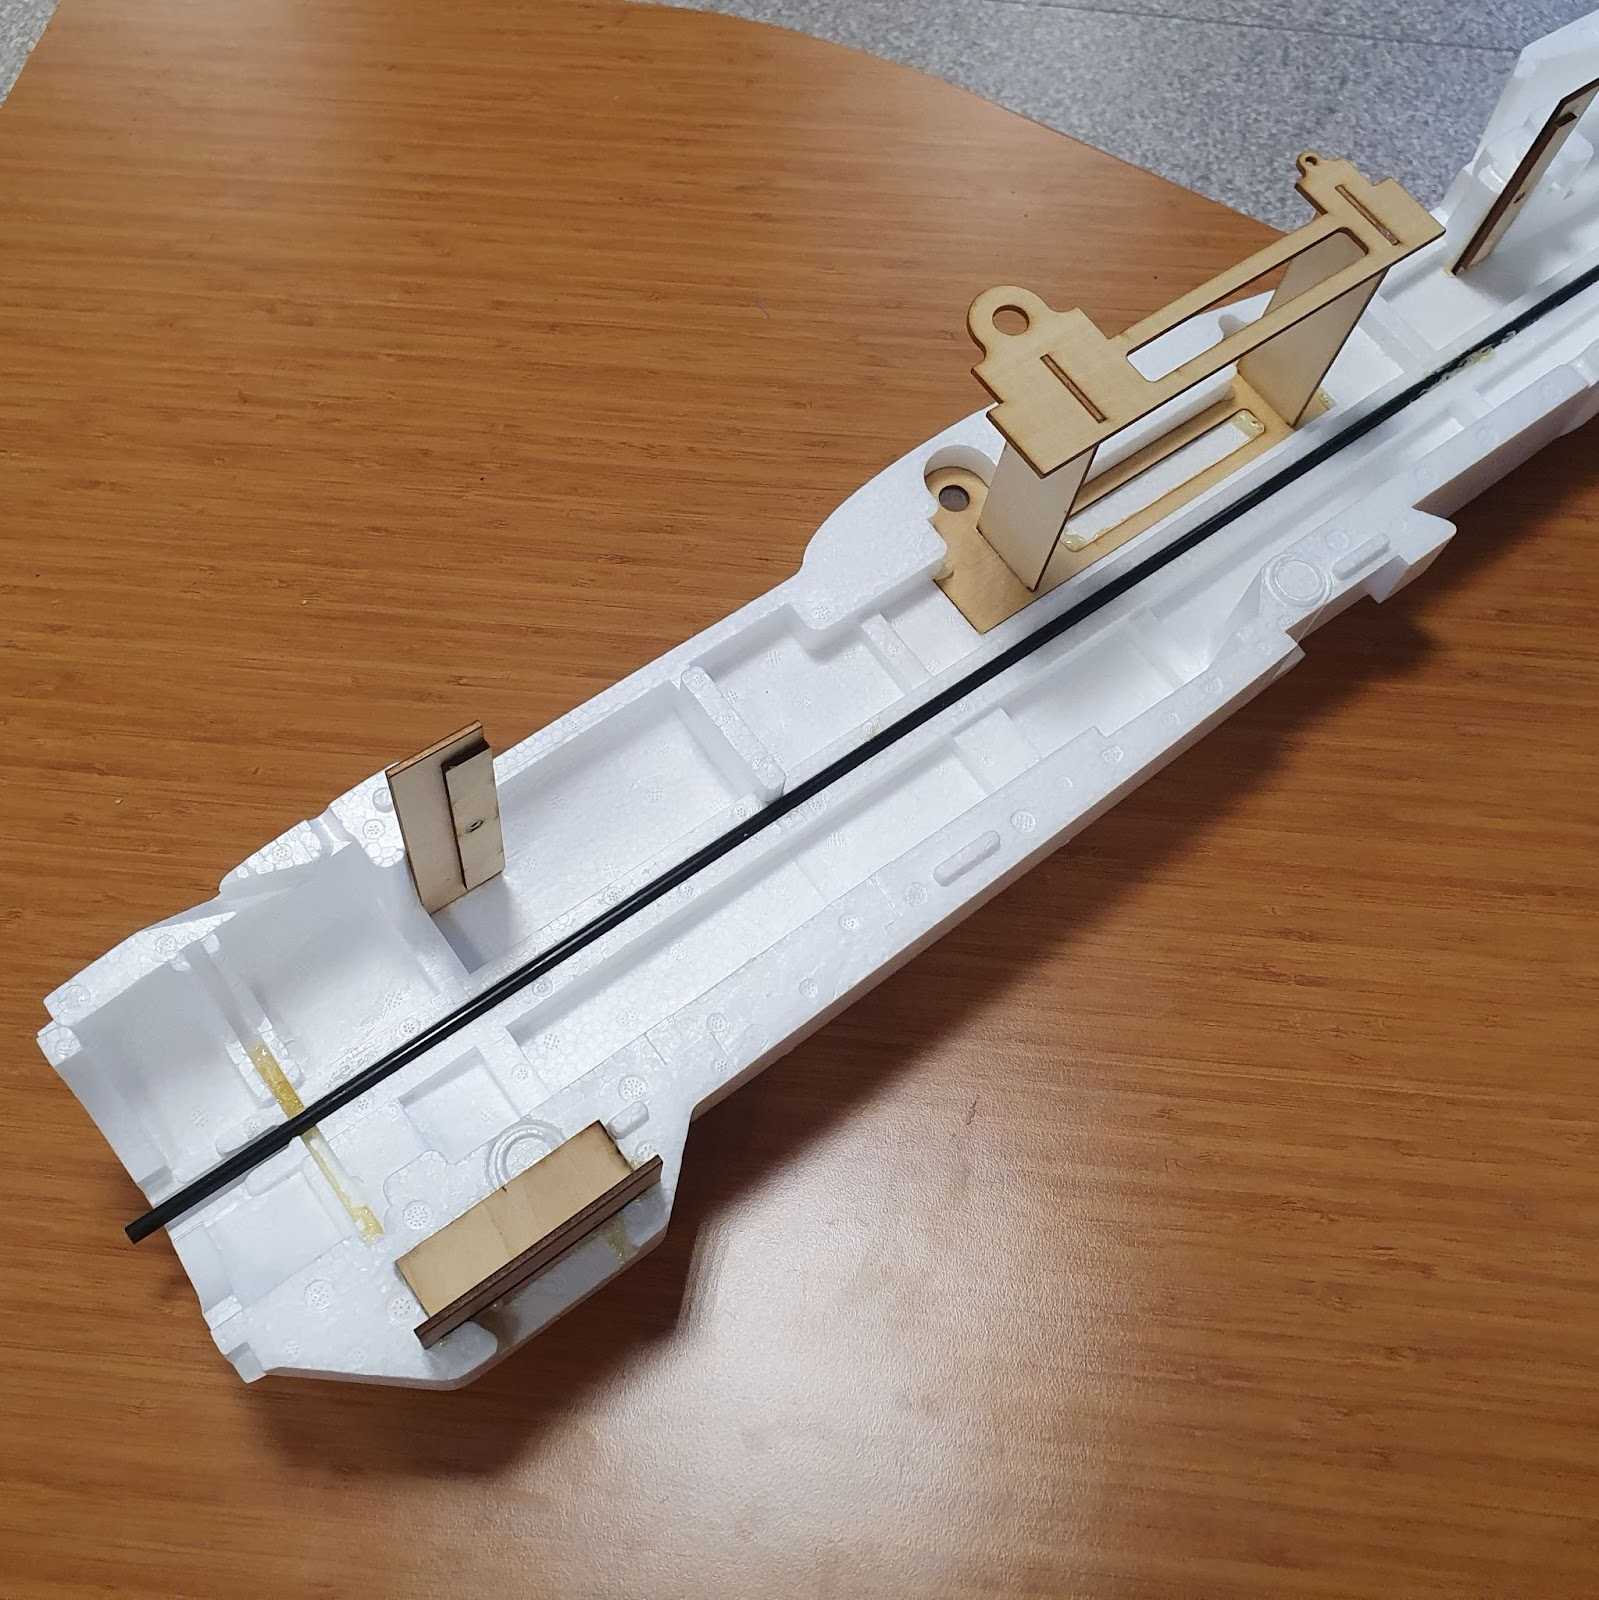
\includegraphics[width=\textwidth]{unnamed (7).jpg}
%       \end{subfigure}
%     \hfill
%     \begin{subfigure}[b]{0.32\textwidth}
%         \centering
%         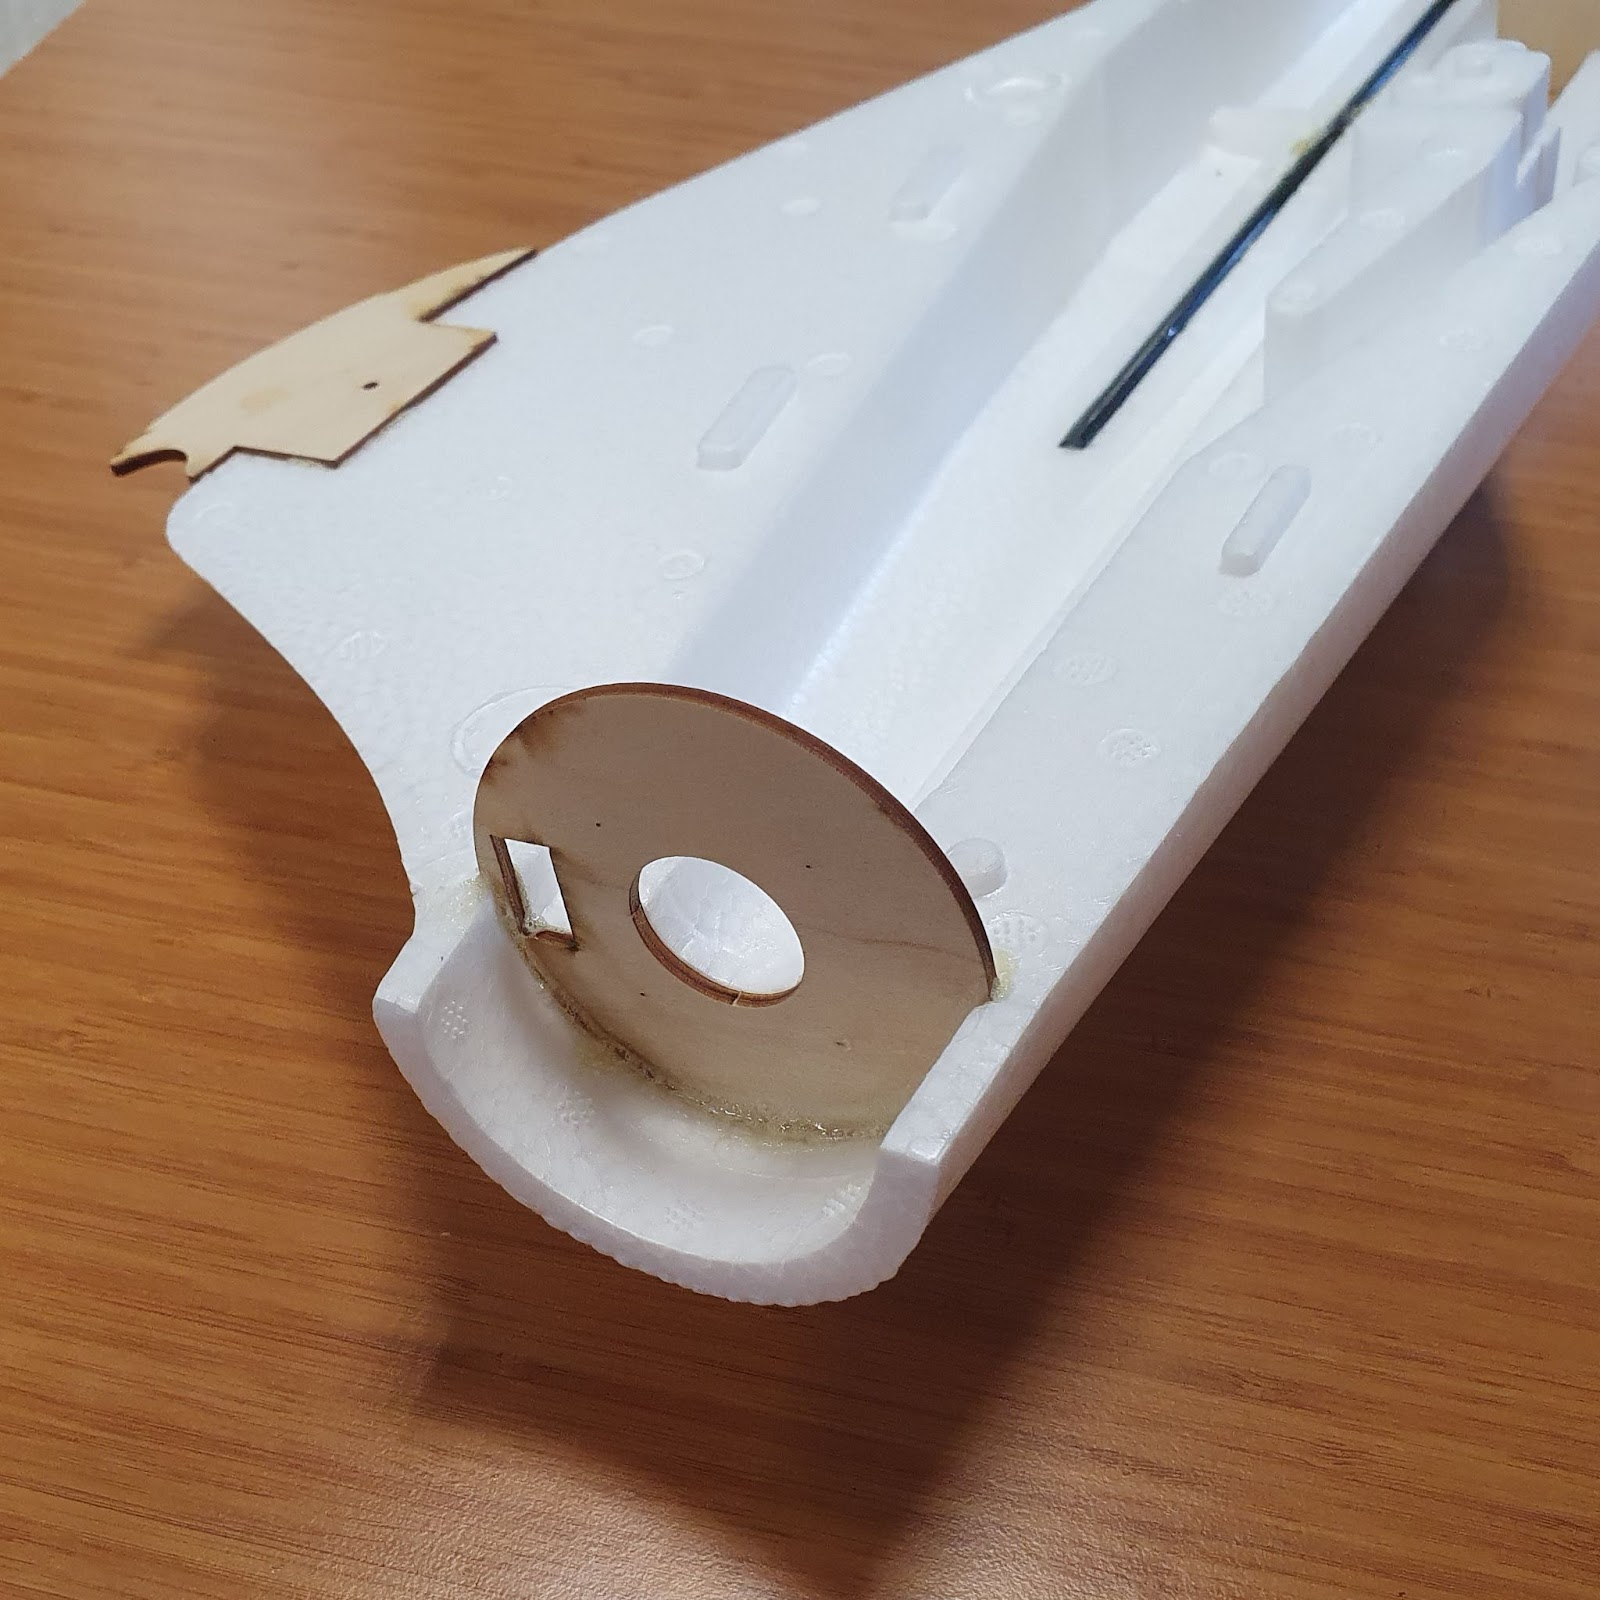
\includegraphics[width=\textwidth]{unnamed (10).jpg}
%     \end{subfigure}
%     \hfill
%     \begin{subfigure}[b]{0.32\textwidth}
%         \centering
%         \includegraphics[width=\textwidth]{unnamed (13).jpg}
%     \end{subfigure}
%     \caption{Assembling the Fuselage}
%    \label{fig:three graphs}
%\end{figure}
%\FloatBarrier

\begin{figure}[ht]
	\centering
	\includegraphics[width = \linewidth]{figures/UAV_assembly.png}
	\caption{Assemblying the UAV}
       \label{fig:assembly}
 \end{figure}
\FloatBarrier
\justify
The wings of the X-UAV Talon are also built from EPO foam. To increase the strength of the wings, carbon fiber rods are glued to the underside of the wing. Plastic clamps are attached to the rods to help with attaching the wings to the fuselage later on. Servo horns are then glued to the control surfaces on the wings and tail. Carbon fiber rods are glued to the tail. Then, the V-Tail is also glued to the fuselage using polyurethane glue.
%\begin{figure}
%     \centering
%     \begin{subfigure}[b]{0.32\textwidth}
%         \centering
%         \includegraphics[width=\textwidth]{unnamed (12).jpg}
%       \end{subfigure}
%     \hfill
%     \begin{subfigure}[b]{0.32\textwidth}
%         \centering
%         \includegraphics[width=\textwidth]{unnamed (11).jpg}
%     \end{subfigure}
%     \hfill
%     \begin{subfigure}[b]{0.32\textwidth}
%         \centering
%         \includegraphics[width=\textwidth]{unnamed (14).jpg}
%     \end{subfigure}
%     \caption{Preparing the Wings}
%    \label{fig:three graphs}
%\end{figure}


\begin{figure}
\centering
    \includegraphics[width=\textwidth]{pre_wing.png}
  \caption{Preparing the Wings}
  \label{Assembled_UAV}
\end{figure}
\FloatBarrier
\justify
After all the parts are properly glued together, the aircraft is ready to be assembled. Assembly of the UAV is fast and user friendly. The wings can be attached to the fuselage using a carbon fiber tube and secured to their places using the plastic clamps inside the wings. The X-UAV Talon can be disassembled into three parts to help with storing and transporting.
 \\
\FloatBarrier


\subsection{Mechanical Integration}
The mechanical integration of our UAV needs careful planning and implementation. Because of the needs of our mission, our UAV has various systems integrated to it. These systems are integrated in a way to be safe, efficient and user friendly. The motor of our aircraft will be mounted to the plywood piece on the rear side in a pusher prop configuration. The ESC that is going to provide power to the motor will be located on the front of the motor and wired to it. The air vents in the rear part of the fuselage will help to keep the ESC cool. The servo motors will be mounted to their places in the wing and the tail. Control rods will be attached between the servo motors and the control horns to connect the control surfaces. The camera of the UAV will be connected to the front plate that lets the camera to have an unobstructed view. \\
\begin{figure}
     \centering
     \begin{subfigure}{0.4\textwidth}
     \centering
        \vfill
        \includegraphics[width=\textwidth]{front_plate.jpg}
         \caption{Front Plate of the UAV}
       \end{subfigure}
     \hspace{2 pt}
     \begin{subfigure}{0.4\textwidth}
         \centering
         \includegraphics[width=\textwidth]{unnamed (17).jpg}
        \caption{Mounting the Servos to the Wings}
     \end{subfigure}
    \label{fig:three graphs}
\end{figure}

\justify
The other parts of the UAV like the computer, battery, flight controller and others will be positioned and secured to their places considering the center of weight of the aircraft. Parts are going to be attached in a way that prevents them from moving while the aircraft is flying. Sensitive equipment will be protected from impact, vibration and other hazards that may damage or harm them.\\

\begin{figure}[ht]
 	\centering
 	\includegraphics[width = .5\linewidth]{motor_tech.jpg}
 	\caption{Technical Drawing of AT3520 Motor\cite{at3520}}
        \label{fig:DC_Motor}
 \end{figure}
\FloatBarrier

\subsection{Electronic Integration}

Although the electronic integration could not be completed due to the ongoing supply of electronic components, how to do it is explained in this section. Electronic integration can be examined under two headings. These are main power line integration and signal line integration.\\

\justify
The maximum current value was taken into account in the cable selection for the integration of the power line. Current breaker and fuse will be placed just after the battery. A POE adapter will be used to provide extra power to the antennaWhile locating the power line cables in the fuselage, care shall be taken to maintain the distance between the cable line and the modules and to ensure that the cable lengths are not excessive in order to ensure that the communication modules are less affected. Attention will be paid to the insulation of the entire power line, especially the soldering areas.\\

\justify
The integration of signal lines, especially the multitude of cables coming to the flight controller, can cause cable tangles. To prevent this, markings will be made on the ends of the cables coming from the servos, ESC, sensors, control receiver, telemetry module, auxiliary computer, which are close to the flight controller. Since the lengths of the internal cables of the servo motors and the ESC will not be sufficient, extension cables will be used. While adjusting the cable lengths, care will be taken to make it easy to put on and take off. Care will be taken to ensure that cable insulation and connectors are not affected by vibration.\\


\section{TEST AND SIMULATION}

\subsection{Sub-System Tests}
\paragraph*{Propulsion Test:} Even though the sufficiency of our propulsion system is calculated theoretically, it is important to test it in real life conditions. An insufficient system can cause our aircraft to behave unexpectedly or it may not satisfy our expectations. After all the elements of the propulsion system are obtained, a thrust test will be made to confirm our calculations. Before the test flight of our UAV, we will confirm that the motor, ESC and the propeller behaves as expected and the maximum thrust they provide is consistent with our calculations.

\paragraph*{Structural Test:} The structural strength and integrity of an aircraft must be tested before it’s flight. The fuselage and the wings of our aircraft will be tested to confirm their strength. To test the wings, it will be supported from its center and then weights will be loaded elliptically, decreasing as we go to the tips of the wing. The weight will be increased gradually until we reach the maximum amount of lift we expect to be generated by the wings. Then, the deviation of the wings will be measured. When we observe that the wings can withstand the weight without deforming permanently, the strength of the wing will be confirmed.

\paragraph*{Telemetry Operation Range Test:} The aim of the test is to measure the range of the telemetry module. The test would be conducted by placing two telemetry modules into a RC drone and installing two ground control stations one of which is close to the RC drone, and the other one is located far from it. One of the telemetry modules would transmit the data of the drone to the close ground control station so that we could obtain the data about the flight. However, the other telemetry module would transmit the data to the ground control station which is located far from it so that we can test when the transmission would be interrupted and determine the maximum range of the telemetry module.

\paragraph*{Artificial Visual Locking Test:} The aim of the test is to measure the accuracy and the latency of the image processing algorithms so that the problems can be detected, and any necessary precaution can be taken. To measure the performance of the algorithm, the onboard camera would be connected to the companion computer in a lab environment, and the camera would be fed by different videos with high frame rates. During this process, the image processing algorithm will be executed on the companion computer and process the data obtained by the camera. At the end of the tests, with the help of the various videos, the accuracy of the algorithm should be examined to detect if the algorithm has any bias towards any particular case. If so, the diversity of the dataset should be improved. The latency of the algorithm should also be measured, and if any problem is spotted, further optimization should be carried out to improve the inference time. 

\paragraph*{Path Following Test:} The aim of this test is to evaluate how much Astrotech UAV deviates from the planned path. By having small increments in time, the difference between planned path and the actual path the Astrotech UAV would cover would be measured, and the accumulation of the error throughout the mission will also be observed. Initially, the test would be carried out in a simulation environment to minimize the risks. After the test in the simulation environment shows the deviation is not that significant, the physical test would be begun.


\subsection{Flight Test and Flight Checklist}
The flight tests planned to be carried out are examined under two headings. The first of these is the tests in which data are collected, or basic autonomous capabilities are checked to understand the flight characteristics of the UAV. These tests are called basic flight tests. The other topic is flight tests for the mission. In these tests, different parts of the software are developed for the competition task, and finally, the task software as a whole is tested. Data from these tests are used for debugging. The following chapters examine basic flight tests in 8.2.1, mission-oriented tests in 8.2.2, and flight checklists in 8.2.3.

\subsubsection{Basic Flight Tests}

\paragraph{First Flight test}

\subparagraph*{Purpose:} The main purpose of this test is to verify that the UAV can fly smoothly in stabilized mode. If the pilot approves after a few laps in the air, then the vehicle's behavior in manual mode is tested. This test will reveal exact details about the flight characteristics of the aircraft while in stabilized mode. It is also required for autotune testing.

\subparagraph*{Procedure:}
Although the first flight is very important in getting to know the UAV, it is one of the flights with the highest risk. Therefore, the flight location and the pilot must be suitable for this in the first flight. Which maneuvers are to be performed after the aircraft takes off and how aggressive to be while performing these maneuvers should be evaluated before the flight. During the test process, the entire test team should follow the flight in anticipation and be ready for any setback. The pilot should assess in advance where he can land in an emergency. 

\justify
There will be no companion computer and camera on the prepared aircraft. This is because these components are not needed for the first flight, and they also increase the loss in case of a possible crash. Pieces of XPS foam of the same weight will be cut and placed in their place.

\justify
After the pre-flight checks are completed, the takeoff step starts. Afterward, maneuvers are made to draw an 8 in the air. These maneuvers are first performed with a large turning radius. A more aggressive turn is expected from the aircraft on each full lap. After observing the aircraft's behavior under this maneuver, different flight modes (LOITER, MANUAL, etc.) and climbing ability at different throttle values can be tested. After the trials are completed, the landing is made.

\paragraph{Autotune} 
\subparagraph*{Purpose:} Controller parameters on the flight control card must be rearranged according to the aircraft used. This arrangement will benefit from the auto-tuning feature of the PX4. After this stage, it is expected that the aircraft will operate more stable in stabilized mode.

\subparagraph*{Procedure:}In this test, the camera and companion computer will not be placed in the aircraft. During the test process, the procedure in the official guide of PX4 will be applied exactly.

\paragraph{Minimum Turning Radius Test}

\subparagraph*{Purpose:} Its calculation is to ensure that the minimum turning radius value, which was made in the 1.2. part and calculated as 9.2 m, is verified using the test data. These values are important as they are important inputs of the control algorithm.

\subparagraph*{Procedure:} In this test, the camera and companion computer will not be placed in the aircraft. 
The 8 maneuvers made in the first flight test will be repeated in this test. After the flight, the position data obtained from the telemetry logs are examined, and a circular fit is applied to the turn curves. The minimum radius value obtained will be used as a constraint in the control software by putting a safety margin on it. While trying to find the correct value as much as possible during detection, a balance will be sought between aggressiveness and reliability regarding control software.

\paragraph{Stall Speed Determination Test}c

\subparagraph*{Purpose:} It is important for the mission how fast the aircraft can go and how low speed it can hold in the air. The stall speed must be determined, especially regarding autonomous landing. This data will be used as the minimum speed constraint in the control software.
The value tried to be determined during this test is for the power-off stall. The test procedure was designed accordingly.

\subparagraph*{Procedure:} In this test, the camera and companion computer will not be placed in the aircraft.
After the pre-flight checks are completed, the UAV will take off and approach the runway repeatedly from a low altitude. During these approaches, the engine will be turned off or run at a very low speed. After these repeated operations, the UAV will land. The telemetry logs obtained will be evaluated, and the speed and heading values will be examined. After the evaluations, the minimum speed constraint to be used in the control software will be determined with the addition of a safety margin.

\paragraph{Autonomous Takeoff Test} 

\subparagraph*{Purpose:} The main purpose of the test is to test the autonomous take-off capability of the UAV.

\subparagraph*{Procedure:} In the autonomous take-off process, which is one of the requirements of the competition, it is expected that the aircraft will take off autonomously after it is thrown by hand. For this, take-off mode from the ground station or remote control will be activated.

\paragraph{Autonomous Landing Test} 

\subparagraph*{Purpose:} The main purpose of the test is to test the autonomous landing capability of the UAV.

\subparagraph*{Procedure:} Autonomous landing is a feature that must be tested as it requires approaching the runway at the right angle and speed. After the landing mode is activated, the behavior of the aircraft will be examined, and accordingly, the change of the relevant parameters or an alternative approach route to the runway will be tried.

\paragraph{Maximum Flight Time Test} 

\subparagraph*{Purpose:} It is to verify that the developed UAV can stay in the air during the mission and the power consumption calculation.

\subparagraph*{Procedure:} All power-consuming components that will be active during the competition must be on the aircraft. At the same time, all these components must be operated at a level close to the power consumption during the mission process. During the flight, the battery voltage variation is observed over the ground station. The descent will be performed when the battery voltage reaches the range of 3.70-3.75 volts. The time between the takeoff command to the aircraft and the UAV's touchdown will be considered the maximum flight time.

\paragraph{Basic Autonomous Flight Test} 

\subparagraph*{Purpose} It is the verification that the UAV can perform autonomous take-off route tracking and autonomous landing successively without any problems.

\subparagraph*{Procedure} Mission planning, one of the features of the PX4 software, will be used during this test. After the final checks, the UAV is thrown by hand and takes off autonomously. It is expected to land autonomously after fulfilling the pre-prepared mission.

\subsubsection[]{Mission-Oriented Flight Tests}

Before starting, some concepts used in this part have to be explained. One of them is a virtual target. A virtual target is the output of the software we have developed. This software creates agents that move like airplanes in 3D space. The initial positions and movements of these agents are random. There are just some predetermined constraints. These are the minimum turning radius, speed, and flight area limits. The software outputs the agents' paths as a list of points. By applying different time filters on this list, it can be adjusted how much detailed information the UAV can get from rival UAVs. Moreover, noise can be added to the output. This concept is an important element that we have designed for use in both simulation studies and field tests. The other concept is the 'path.' The path can be a curve or a list of points in three-dimensional space. Its distinguishing feature is that it can be tracked by a fixed-wing aircraft.
\begin{figure}
     \centering
     \begin{subfigure}{0.4\textwidth}
     \centering
        \vfill
        \includegraphics[width=\textwidth]{figures/unnamed (29).png}
         \caption{Front Plate of the UAV}
       \end{subfigure}
     \hspace{2 pt}
     \begin{subfigure}{0.4\textwidth}
         \centering
         \includegraphics[width=\textwidth]{figures/unnamed (30).png}
        \caption{Mounting the Servos to the Wings}
     \end{subfigure}
    \label{fig:three graphs}
\end{figure}


\paragraph{Previously Generated Path Following Test} 

\subparagraph*{Purpose:} The element to be tested in this test is to follow a specific path with commands from the companion computer. This test is a requirement for editing the parameters of the control software (e.g. look ahead distance).

\subparagraph*{Procedure:}

All subsequent tests are based on the procedure of the basic autonomous flight test. The only change is that the task software on the auxiliary computer will be run by switching to off-board mode instead of PX4 missions.

\justify
The control software on the companion computer on the UAV will be set to follow the path given to it as a list of points. This path will be drawn considering the flight characteristics of the aircraft. It will be tested whether the UAV can follow this path by flying in off-board mode. The UAV is expected to follow the path with the least deviation.

\paragraph{Approaching Test with Single Virtual Target}

\subparagraph*{Purpose:} In this test, the UAV's target selection and its decision to unfollow the target when necessary will be tested. 

\subparagraph*{Procedure:} The test will be performed on the test infrastructure used in the Geo-Fencing test. During the test process, data of more than one virtual target is sent instead of one in the data package sent to the UAV. These targets are created with different starting positions and all move randomly. Target selection and tracking success of the UAV are evaluated. This test is one of the tests that is planned to be repeated the most.

\paragraph{Approaching and Locking Test with Real Target}
\subparagraph*{Purpose:} Integrated testing of the approach and lock parts of the mission 

\subparagraph*{Procedure:} A number of modifications are required for this test at the ground station. First of all, the Wi-Fi module used in image transmission, which was not needed until now, has to be installed for this test. In order to transfer the data from the target UAV to the ground station, one more telemetry module must be used. The data coming to the ground station from the target UAV is filtered and transferred to the Astrotech UAV. In line with these data, the tracking algorithm of the UAV and the operation of the visual-based guidance software are examined.  The pilot should be cautious as there is a possibility of air collision during the test process.

\paragraph{Kamikaze Mission Test}

\subparagraph*{Purpose:}
It is to verify that the UAV can perform its kamikaze mission. In order to fulfill this task, it must perform the diving maneuver without any problems. The camera should be affected by vibrations as little as possible while reading the QR code while diving.

\subparagraph*{Procedure:} The test will be carried out in two stages since the risk of slaughter is high. In the first stage, the auxiliary computer and camera will not be on the UAV. Equi-weighted foam pieces will be placed in their place. What is being tested at this stage is the success of the diving maneuver. In the second phase, these components will be placed in place and the mission will be tested as a whole.
In the first stage, the UAV starts to navigate at the highest altitude that will comply with the relevant regulation of the General Directorate of Civil Aviation (SHGM) after take-off. From this altitude, it makes a dive maneuver towards the determined ground target. The maneuver should be shorter and less aggressive at first attempts. The acuity of the maneuvers and the dive distance are increased until they meet the requirements of the mission. Diving distance stands out as it will increase the time that can be used to read the QR code.
In the second stage, the camera is actively locked to the ground target. Recognition of the QR code (or another visible target) and sending the corresponding data packet to the ground are tested.
Since it is one of the tests with a high risk of slaughter, it requires additional considerations. Considering the dive height and speed of the aircraft, the test team should make sure that there is no one within 100 meters of the center of the diving area. Other points to be considered are that the target area should be an earth ground, if possible, and that it should be free of elements that could increase the loss at the time of a crash in the area.

\paragraph{Simulations:} The tests carried out in the simulation environment can be thought of as a projection of the tests planned to be carried out in the field in a virtual environment. In these tests, PX4-SITL is run with Gazebo simulation environment with standard plane model and RTPS turned on. In this way, both uORB messaging over ROS2 nodes, and MAVLink messaging using MAVSDK can be performed. In addition, snapshots from the aircraft model in the simulation environment can also be processed by transferring them to a ROS2 node.
\justify
All mission-oriented tests will not be performed in the field without being tested once in this simulation environment. The test procedures will be finalized in line with the observations made in the simulations.

\subsubsection{Flight Checklist}
The flight checklist is a point that is highly valued by our team. Since there are many details to be considered during the flight process, it requires careful work.

\justify
The checklist given below contains items for the 4 main stages. These can be listed as what to do before going to the flight area, at the flight area, what to do just before the flight, and after.

\justify
In addition, the red or yellow color was preferred for each item. While the red color is used for the items that may directly cause the flight not to take place or the flight safety to be at risk, the yellow color is used for the mission-specific items.
\begin{table}[ht]
	\centering
	\includegraphics[width = .9\linewidth]{figures/checklist.png}
	\caption{Flight Checklist}
       \label{fig:checklist}
 \end{table}

\FloatBarrier
\section{SAFETY}
 Safety is one of the most important aspects of every project. During the production of our UAV, there are steps that can be potentially hazardous to the team members. Because of that, we give utmost importance to safety precautions. Our team members are informed about the tools we use and aware of the possible dangers. To create a safe working environment, necessary equipment such as goggles and gloves are used especially during the manufacturing phase. We also have a fire extinguisher and first aid kit in our workplace in case of any emergency. 
 
 \justify
The Li-Po battery used in our UAV as a power supply can be hazardous for various reasons. One of the common reasons is ignition while charging. Therefore, Li-Po batteries are kept in storage bags made of fireproof fabric to prevent fire in our workplace. Another safety precaution is related to the propeller of the Astrotech UAV, which can spin at dangerously high speeds and pose a danger to our team members. To prevent any hazard, the propeller would be mounted just before flights. Additionally, the engine would be shut down just before the landing to prevent the propellers from hitting the ground and breaking apart. Also, there is a wooden piece at the back of the Astrotech UAV which can be seen in Figure \ref{fig:piece}. This piece provides a soft landing and protects the person holding the Astrotech UAV from propeller related accidents during take-off.

\begin{figure}[ht]
 	\centering
 	\includegraphics[width = .5\linewidth]{safety.png}
 	\caption{Plywood protection piece.}
 	\label{fig:piece}
 \end{figure}
\FloatBarrier
\clearpage 
\section{REFERENCES}

\singlespacing
\bibliographystyle{IEEEtran} 
\bibliography{references}
\end{document}